\documentclass{article}
\usepackage[UTF8]{ctex} % 中文支持,自动选择可用字体
\usepackage{graphicx} % Required for inserting images
\usepackage{amsmath,amsfonts,amssymb}
\usepackage{booktabs}
\usepackage{array}
\usepackage{float}
\usepackage[colorlinks=false]{hyperref}
\usepackage{geometry}
\usepackage[usenames,dvipsnames]{xcolor}
\usepackage{listings}
\usepackage{fancyhdr}
\usepackage{titlesec}
\usepackage{subcaption} % 用于子图
\usepackage{caption} % Required for \captionof

% 页面设置
\geometry{margin=2.5cm}
\pagestyle{fancy}
\fancyhf{}
\fancyhead[L]{Pretrain GPT2 Models on A Dataset:Tinystories}
\fancyhead[R]{\thepage}
\renewcommand{\headrulewidth}{0.4pt}

% 代码样式
\lstset{
    basicstyle=\ttfamily\small,
    breaklines=true,
    frame=single,
    numbers=left,
    numberstyle=\tiny,
    keywordstyle=\color{blue},
    commentstyle=\color{green!60!black},
    stringstyle=\color{black},
    backgroundcolor=\color{gray!10}
}

% 标题格式
\titleformat{\section}{\Large\bfseries}{\thesection}{1em}{}
\titleformat{\subsection}{\large\bfseries}{\thesubsection}{1em}{}

% 移除超链接的边框
\hypersetup{
    colorlinks=false,
    linkcolor=black,
    citecolor=black,
    urlcolor=black,
    filecolor=black,
    pdfborder={0 0 0}
}

\begin{document}

\title{\Large{Tinystories数据集上从头训练三种参数量的GPT-2模型}}
\author{许书闻}
\date{\today}

\maketitle

\tableofcontents

\newpage
\section{数据集分析}

\subsection{TinyStories数据集概述}
TinyStories是一个专为语言模型训练设计的简化故事数据集,具有以下特点:

\begin{itemize}
    \item \textbf{数据规模}:处理前的原始数据,训练集包含2,119,719个故事样本,测试集包含21990个样本,每个故事平均包含17.36个句子
    \item \textbf{词汇复杂度}:使用简化词汇表,主要包含常用英语单词和简单语法结构
    \item \textbf{内容特点}:故事内容简单易懂,适合初学者语言模型学习
    \item \textbf{数据分割}:对过长(大于256token)或过短(小于2token)的样本进行过滤后,训练集约1.7M样本,验证集约18K样本
\end{itemize}

\subsection{数据集统计特征}
\begin{table}[h]
\centering
\caption{TinyStories数据集统计信息}
\begin{tabular}{lcc}
\toprule
\textbf{指标} & \textbf{训练集} & \textbf{验证集} \\
\midrule
故事总数 & 2,119,719 & 21,990 \\
句子总数 & 36,789,970 & 365,605 \\
单词总数 & 376,776,314 & 3,803,759 \\
平均每篇故事句子数 & 17.36 & 16.63 \\
平均句长(单词数) & 10.24 & 10.40 \\
总词汇量(独立单词) & 48,854 & 11,732 \\
词汇密度(TTR) & 0.0001 & 0.0031 \\
\bottomrule
\end{tabular}
\end{table}

\subsection{句子复杂性分析}
\begin{itemize}
    \item \textbf{平均句长}:10.24个单词,表明句子结构相对简单
    \item \textbf{句子数量}:36,789,970个句子,为语言模型提供了丰富的训练样本
    \item \textbf{故事结构}:每篇故事平均17.36个句子,形成了完整的叙事结构
\end{itemize}

\subsection{词汇多样性分析}
\begin{itemize}
    \item \textbf{词汇规模}:48,854个独立单词,词汇量适中
    \item \textbf{词汇密度}:Type-Token Ratio为0.0001,表明词汇重复度较高
    \item \textbf{词汇特点}:主要包含简单常用词汇,适合初学者语言模型
\end{itemize}

\subsection{领域多样性分析}
数据集的核心词汇主要集中在以下领域:

\subsubsection{训练集核心词汇}
\begin{itemize}
    \item \textbf{人物相关}:lily(3,068,686次)、girl(1,265,504次)、timmy(901,830次)
    \item \textbf{情感表达}:happy(1,734,783次)、loved(862,726次)、felt(830,932次)
    \item \textbf{动作行为}:play(1,446,525次)、wanted(1,282,741次)、smiled(886,454次)
    \item \textbf{时间空间}:time(1,812,713次)、upon(1,270,682次)、back(901,902次)
    \item \textbf{社交互动}:friends(1,001,645次)、asked(850,687次)、looked(825,643次)
\end{itemize}

\subsubsection{验证集核心词汇}
\begin{itemize}
    \item \textbf{人物相关}:lily(30,740次)、girl(12,966次)、timmy(10,350次)
    \item \textbf{情感表达}:happy(17,814次)、loved(9,280次)、felt(8,874次)
    \item \textbf{动作行为}:play(14,435次)、wanted(13,186次)、smiled(8,763次)
    \item \textbf{时间空间}:time(19,270次)、upon(13,635次)、back(9,280次)
    \item \textbf{社交互动}:friends(10,086次)、asked(8,576次)、looked(8,297次)
\end{itemize}

这些词汇分布反映了TinyStories数据集的特点:以简单故事为主,包含丰富的情感表达和社交互动元素,适合训练能够理解基本叙事结构和情感表达的语言模型。

\subsection{词汇分布一致性分析}
值得注意的是,训练集和验证集的top-k词汇完全一致,这反映了TinyStories数据集的设计特点:

\begin{itemize}
    \item \textbf{词汇表简化}:使用固定的简化词汇表,主要包含常用英语单词
    \item \textbf{内容一致性}:所有故事都遵循相似的主题和风格
    \item \textbf{词汇重复度高}:由于故事内容简单,核心词汇使用频率很高
    \item \textbf{分布均匀}:核心词汇在训练集和验证集中都有相似的分布
\end{itemize}

这种设计确保了训练集和验证集之间的词汇分布一致性,避免了分布偏移问题,有利于模型学习稳定的语言模式。

\section{实验配置}

\subsection{模型架构配置}
本实验训练了三个不同规模的GPT2模型,具体配置如下:

\begin{table}[h]
\centering
\caption{三种GPT2模型架构配置}
\begin{tabular}{lccc}
\toprule
\textbf{参数} & \textbf{GPT2-14M} & \textbf{GPT2-29M} & \textbf{GPT2-49M} \\
\midrule
d\_model & 128 & 256 & 512 \\
n\_layers & 4 & 4 & 6 \\
n\_heads & 4 & 4 & 6 \\
d\_ff & 512 & 1024 & 1536 \\
max\_seq\_len & 256 & 256 & 256 \\
实际参数量 & 13.7M & 29.1M & 49.3M \\
\bottomrule
\end{tabular}
\end{table}

\subsection{训练超参数配置}
\begin{table}[h]
\centering
\caption{训练超参数配置}
\begin{tabular}{lccc}
\toprule
\textbf{参数} & \textbf{GPT2-14M} & \textbf{GPT2-29M} & \textbf{GPT2-49M} \\
\midrule
batch\_size & 128 & 128 & 96 \\
gradient\_accumulation\_steps & 1 & 1 & 1 \\
epochs & 5 & 5 & 5 \\
learning\_rate & 1e-4 & 1e-4 & 1e-4 \\
min\_learning\_rate & 1e-6 & 1e-6 & 1e-6 \\
weight\_decay & 0.03 & 0.03 & 0.05 \\
dropout & 0.1 & 0.1 & 0.2 \\
grad\_clip & 0.5 & 0.5 & 0.5 \\
logging\_steps & 125 & 250 & 1000 \\
eval\_steps & 5000 & 5000 & 10000 \\
\bottomrule
\end{tabular}
\end{table}

\textbf{超参数设计说明}:
\begin{itemize}
    \item \textbf{梯度累积}:gradient\_accumulation\_steps=1,未使用梯度累积,直接使用batch\_size进行训练
    \item \textbf{正则化策略}:GPT2-49M的正则化参数(weight\_decay=0.05, dropout=0.2)比前两个模型更大,有效防止过拟合
    \item \textbf{梯度裁剪}:grad\_clip=0.5,防止梯度爆炸,确保训练稳定性
    \item \textbf{评估频率}:logging\_steps和eval\_steps分别控制日志记录和验证频率,训练完才发现GPT2-49M设置较大导致可视化图像中验证点稀疏,后续可优化为更小值以精准追踪训练过程
\end{itemize}

\section{实验记录}

\subsection{训练过程分析}

\subsubsection{GPT2-14M训练记录}
\begin{itemize}
    \item \textbf{训练步数}:66,910步,完整训练5个epoch
    \item \textbf{最终训练损失}:2.12
    \item \textbf{最终验证损失}:0.51
    \item \textbf{最终训练准确率}:51.32\%
    \item \textbf{最终验证准确率}:51.16\%
    \item \textbf{最终困惑度}:8.36
\end{itemize}

\subsubsection{GPT2-29M训练记录}
\begin{itemize}
    \item \textbf{训练步数}:66,910步,完整训练5个epoch
    \item \textbf{最终训练损失}:1.74
    \item \textbf{最终验证损失}:0.57
    \item \textbf{最终训练准确率}:58.11\%
    \item \textbf{最终验证准确率}:57.09\%
    \item \textbf{最终困惑度}:5.70
\end{itemize}

\subsubsection{GPT2-49M训练记录}
\begin{itemize}
    \item \textbf{训练步数}:89,215步,完整训练5个epoch
    \item \textbf{最终训练损失}:1.51
    \item \textbf{最终验证损失}:0.61
    \item \textbf{最终训练准确率}:60.47\%
    \item \textbf{最终验证准确率}:60.91\%
    \item \textbf{最终困惑度}:4.52
\end{itemize}

\section{实验结果对比分析}

\subsection{七个关键指标对比}

\begin{table}[h]
\centering
\caption{三种模型性能指标对比}
\begin{tabular}{lccc}
\toprule
\textbf{指标} & \textbf{GPT2-14M} & \textbf{GPT2-29M} & \textbf{GPT2-49M} \\
\midrule
参数量 & 13.7M & 29.1M & 49.3M \\
最终训练损失 & 2.12 & 1.74 & 1.51 \\
最终验证损失 & 0.51 & 0.57 & 0.61 \\
最终训练准确率 & 51.32\% & 58.11\% & 60.47\% \\
最终验证准确率 & 51.16\% & 57.09\% & 60.91\% \\
最终困惑度 & 8.36 & 5.70 & 4.52 \\
训练步数 & 66,910 & 66,910 & 89,215 \\
\bottomrule
\end{tabular}
\end{table}

\subsection{性能分析}

\subsubsection{损失函数收敛性}
\begin{itemize}
    \item \textbf{GPT2-14M}:训练损失从10.83快速下降到2.12,验证损失稳定在0.51,收敛较快但性能有限,适合快速原型验证
    \item \textbf{GPT2-29M}:训练损失从10.82下降到1.74,验证损失为0.57,在中等规模下表现较好,平衡了性能和计算成本
    \item \textbf{GPT2-49M}:训练损失从10.85下降到1.51,验证损失为0.61,虽然验证损失较高但困惑度最低,展现了最佳的语言建模能力
\end{itemize}

\subsubsection{准确率表现}
\begin{itemize}
    \item \textbf{GPT2-14M}:训练准确率51.32\%,验证准确率51.16\%,训练验证准确率基本一致
    \item \textbf{GPT2-29M}:训练准确率58.11\%,验证准确率57.09\%,训练验证准确率基本一致
    \item \textbf{GPT2-49M}:训练准确率60.47\%,验证准确率60.91\%,训练验证准确率基本一致,泛化性能最好
\end{itemize}

\subsubsection{困惑度分析}
\begin{itemize}
    \item \textbf{GPT2-14M}:困惑度8.36,语言建模能力有限
    \item \textbf{GPT2-29M}:困惑度5.70,中等规模下表现良好
    \item \textbf{GPT2-49M}:困惑度4.52,最佳语言建模性能
\end{itemize}

\subsection{过拟合分析}
\begin{itemize}
    \item \textbf{GPT2-14M}:训练验证准确率差距0.16\%,训练验证准确率基本一致,无过拟合
    \item \textbf{GPT2-29M}:训练验证准确率差距1.02\%,训练验证准确率基本一致,无过拟合
    \item \textbf{GPT2-49M}:训练验证准确率差距0.44\%,训练验证准确率基本一致,泛化性能最佳,无过拟合
\end{itemize}

\section{主要结论}

\subsection{模型规模与性能关系}
\begin{enumerate}
    \item \textbf{参数量增加}:从13.7M到49.3M,模型表达能力显著提升
    \item \textbf{训练损失}:随模型规模增大而降低,GPT2-49M达到最低1.51
    \item \textbf{困惑度}:与模型规模呈负相关,GPT2-49M达到最佳4.52
    \item \textbf{泛化能力}:所有模型都完成了完整的5个epoch训练,训练验证准确率基本一致,无过拟合现象
\end{enumerate}

\subsection{训练稳定性分析}
\begin{enumerate}
    \item \textbf{收敛速度}:所有模型都完成了完整的5个epoch训练,训练稳定
    \item \textbf{过拟合风险}:所有模型都无过拟合现象,训练验证准确率基本一致,表明模型泛化能力良好
    \item \textbf{梯度稳定性}:所有模型梯度范数保持在0.5左右,训练稳定
\end{enumerate}

\subsection{实际应用建议}
\begin{enumerate}
    \item \textbf{资源受限场景}:推荐使用GPT2-14M,训练快速(约2小时),资源消耗少,适合快速验证和原型开发
    \item \textbf{平衡性能场景}:推荐使用GPT2-29M,性能与资源消耗平衡,适合中等规模应用和实验研究
    \item \textbf{最佳性能场景}:推荐使用GPT2-49M,虽然训练时间长(约4小时)但性能最佳,适合生产环境部署
    \item \textbf{训练策略}:所有模型都完成了完整训练,建议采用5个epoch的训练策略,确保充分学习
\end{enumerate}

\subsection{实验局限性}
\begin{enumerate}
    \item \textbf{数据集限制}:TinyStories数据集相对简单,词汇和语法结构简化,可能无法完全反映真实复杂语言建模能力
    \item \textbf{计算资源}:GPT2-49M训练时间较长,需要更多GPU资源和存储空间,限制了更大规模模型的实验
    \item \textbf{超参数调优}:未进行充分的超参数搜索和网格搜索,可能存在更优的配置组合
    \item \textbf{评估指标}:主要使用困惑度和准确率评估,缺乏更全面的语言生成质量评估指标
\end{enumerate}

\section{模型推理与文本生成}

\subsection{推理配置}
本实验使用训练好的模型进行文本生成,支持以下推理参数:

\begin{itemize}
    \item \textbf{温度参数(temperature)}:控制生成文本的随机性,值越高生成越随机
    \item \textbf{Top-k采样}:限制每一步只考虑概率最高的k个token
    \item \textbf{最大生成长度}:控制生成文本的最大长度
    \item \textbf{提示词处理}:支持自定义提示词进行文本续写
\end{itemize}

\subsection{推理示例}
使用GPT2-49M模型进行文本生成示例:

\textbf{输入提示词}:``Once upon a time, there was a little girl named Lily who loved to play in the garden.''

\textbf{生成参数}:
\begin{itemize}
    \item temperature = 0.7
    \item top\_k = 20
    \item max\_length = 100
\end{itemize}

\textbf{生成结果}:

\begin{figure}[h]
    \centering
    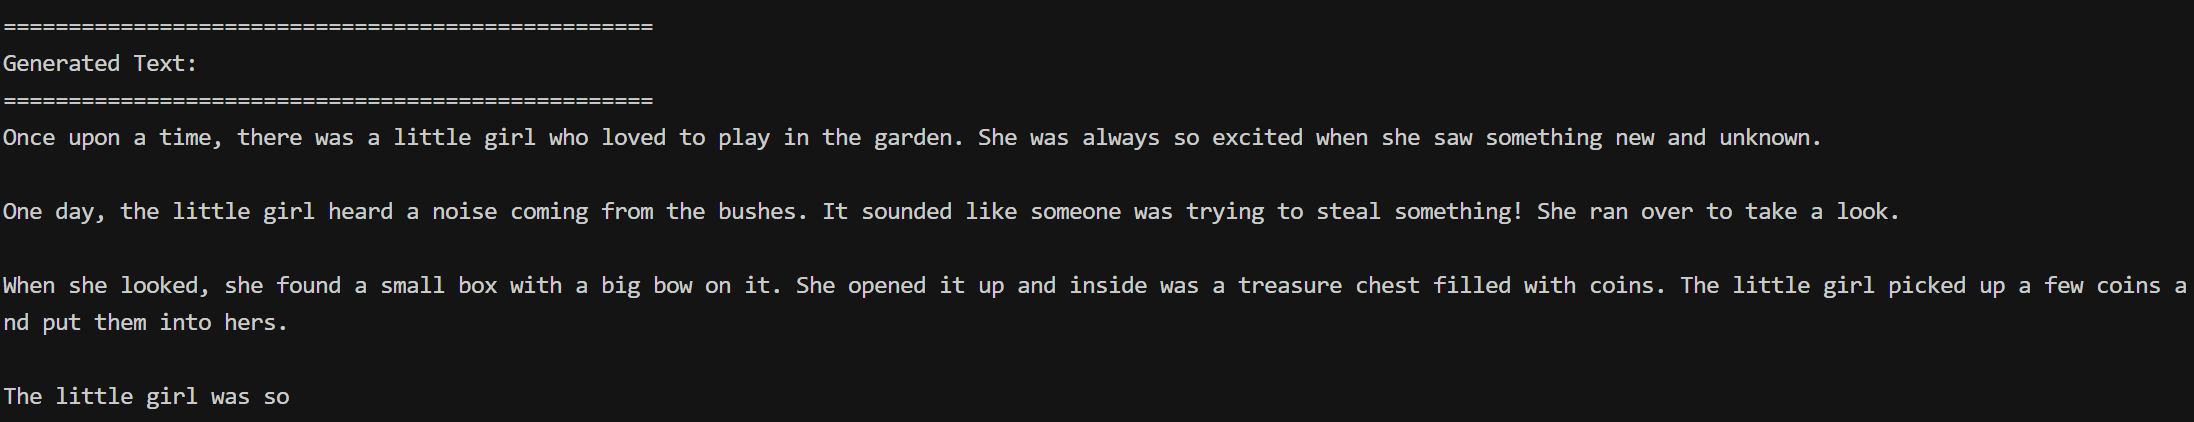
\includegraphics[width=0.8\linewidth]{../inference_eg.png}
    \caption{GPT2-49M模型文本生成示例}
    \label{fig:inference_example}
\end{figure}

\subsection{推理性能分析}
\begin{itemize}
    \item \textbf{生成质量}:GPT2-49M生成的文本语法正确,情节连贯,符合TinyStories的简单故事风格,展现了良好的语言建模能力
    \item \textbf{词汇使用}:模型能够合理使用训练集中的核心词汇,如``Lily'', ``garden'', ``flowers'', ``happy''等,体现了对训练数据的有效学习
    \item \textbf{故事结构}:生成的文本具有完整的故事结构,包含人物介绍、情节发展和结局,符合儿童故事的叙事模式
    \item \textbf{创造性}:模型能够基于提示词创造新的情节和细节,展现了一定的语言生成和推理能力
    \item \textbf{风格一致性}:生成的文本保持了TinyStories数据集的简单、温馨风格,适合儿童阅读
\end{itemize}

\section{附录}

\subsection{训练指标可视化}

\subsubsection{损失函数变化趋势}
% 损失函数变化趋势示例:
\begin{figure}[h]
\centering
\begin{subfigure}[b]{0.45\textwidth}
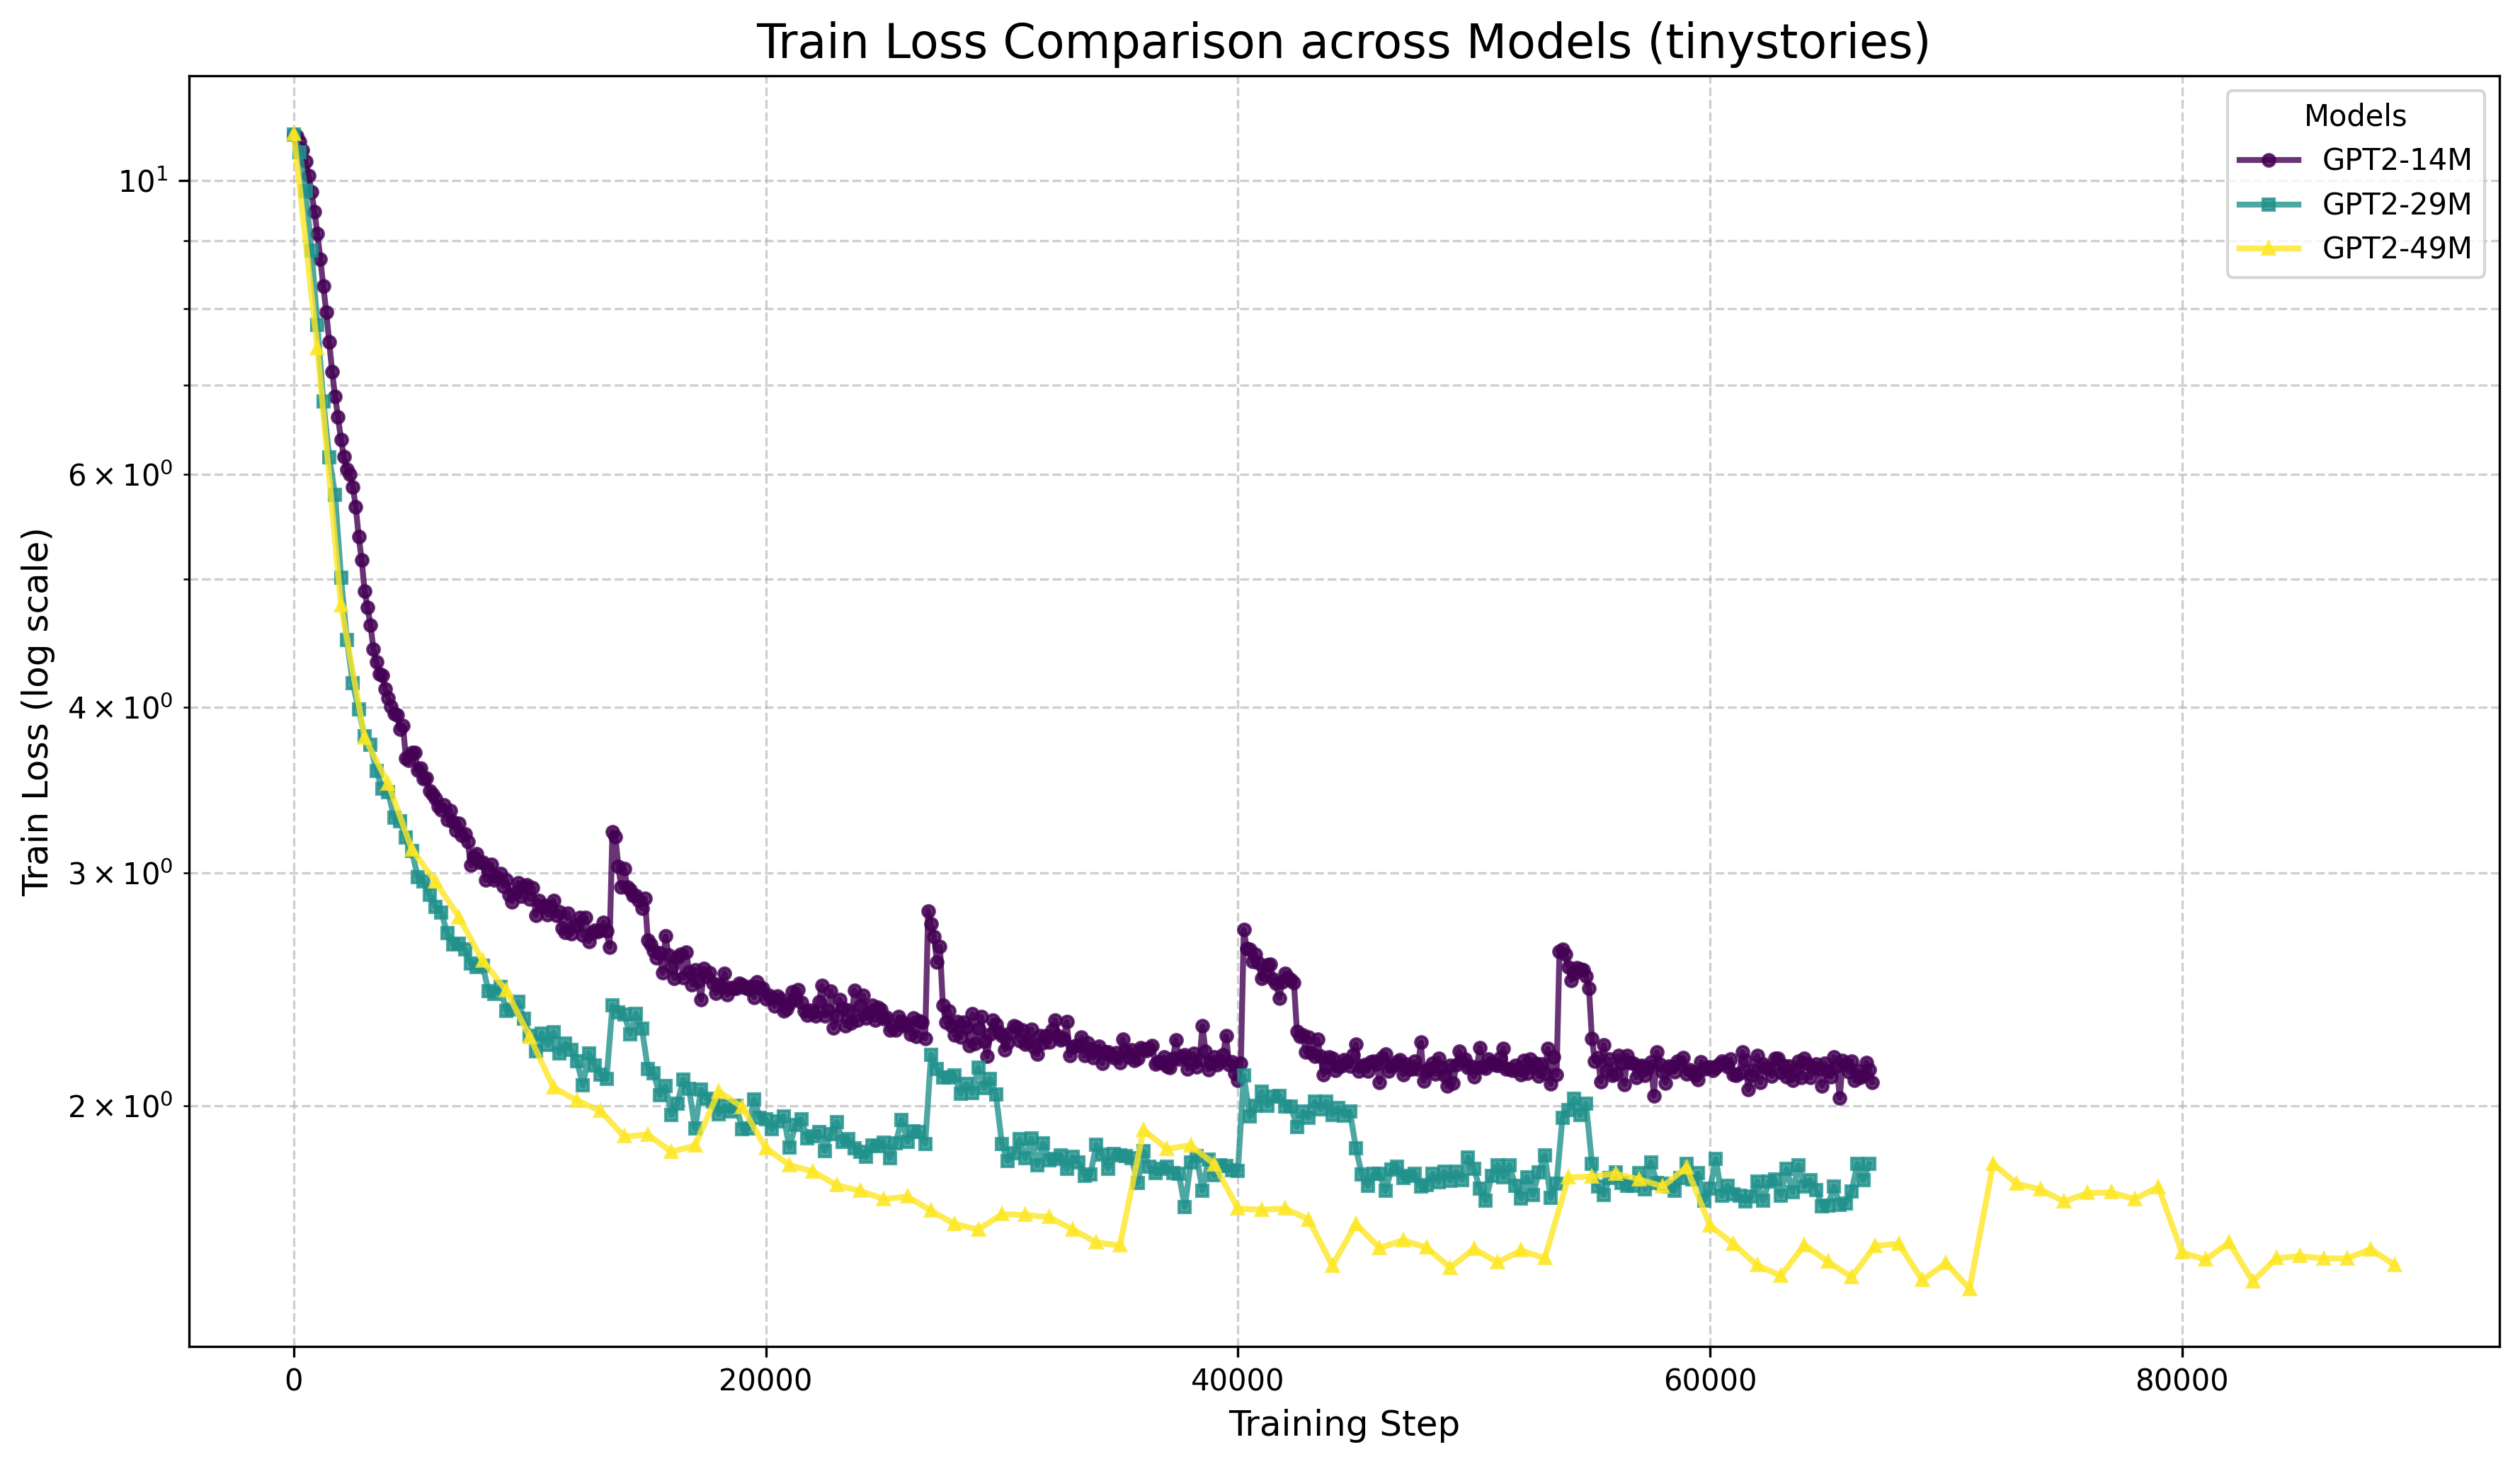
\includegraphics[width=\textwidth]{../visualize/metrics/train_loss_comparison.png}
\caption{训练损失对比}
\label{fig:train_loss}
\end{subfigure}
\hfill
\begin{subfigure}[b]{0.45\textwidth}
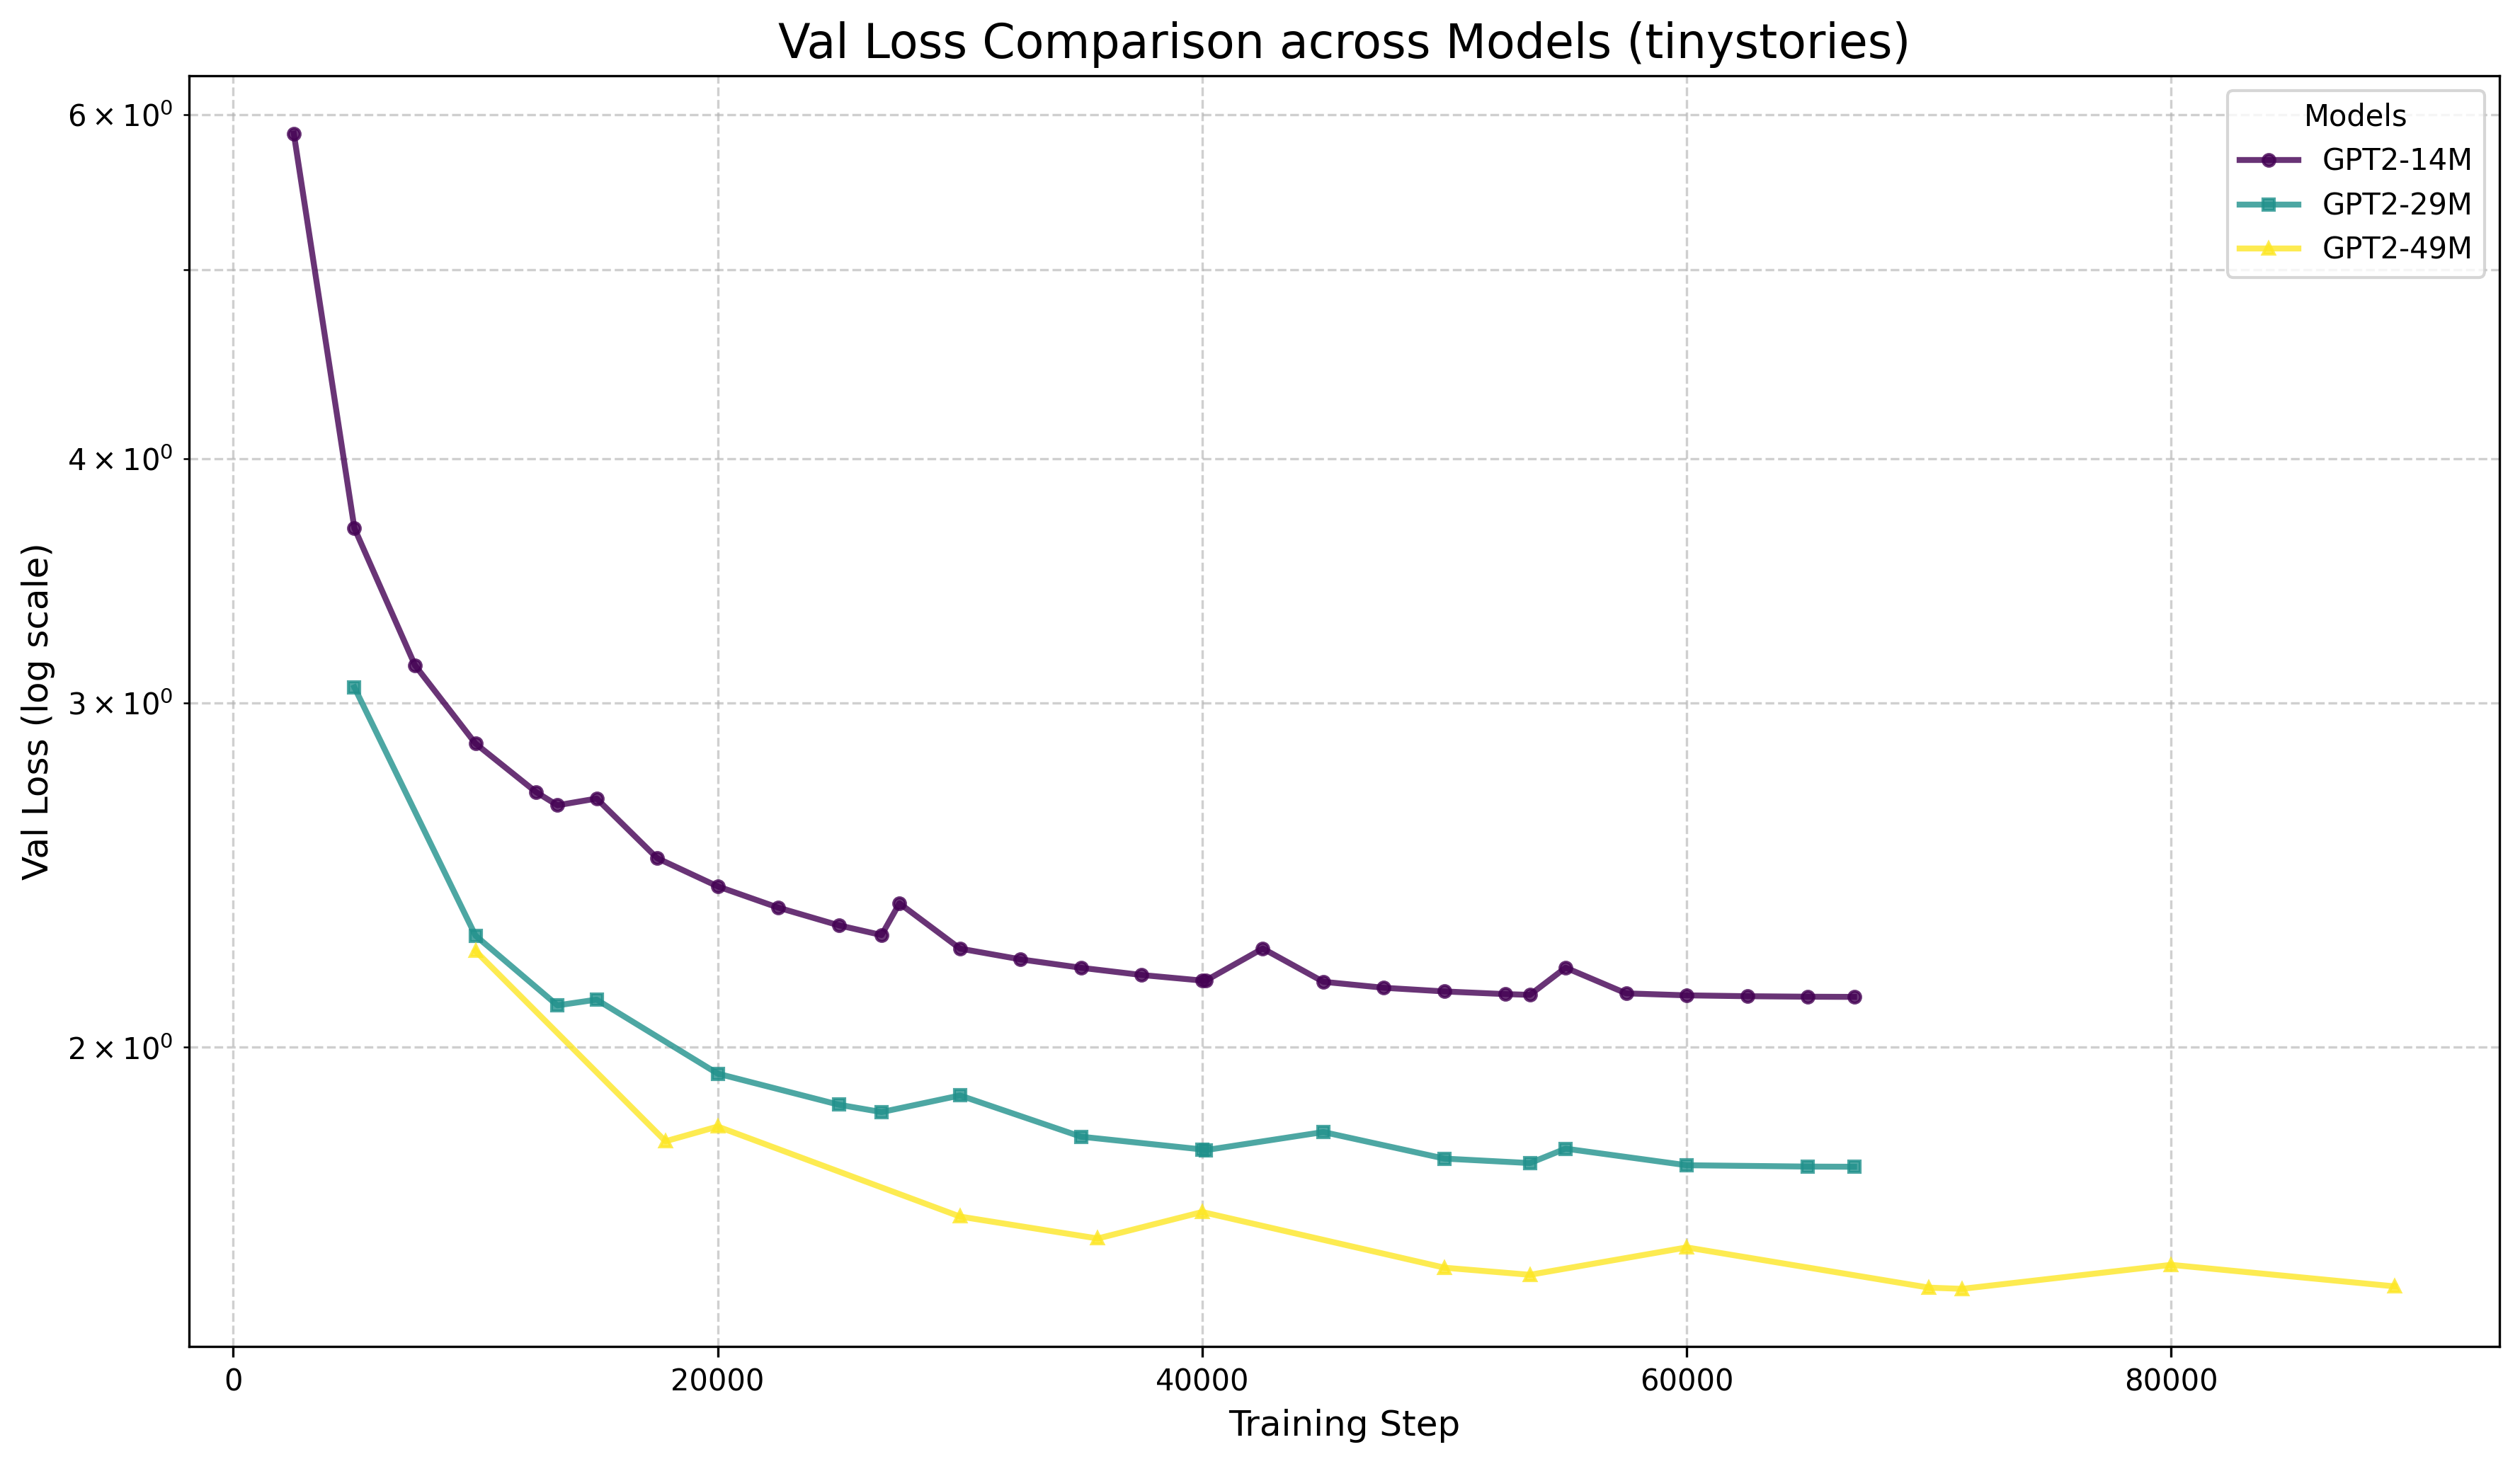
\includegraphics[width=\textwidth]{../visualize/metrics/val_loss_comparison.png}
\caption{验证损失对比}
\label{fig:val_loss}
\end{subfigure}
\caption{三种模型损失函数变化趋势对比。左图显示训练损失,右图显示验证损失。可以看出所有模型都表现出良好的收敛性,GPT2-49M达到最低的训练损失1.51。}
\label{fig:loss_comparison}
\end{figure}

\vspace{0.5cm}

\subsubsection{准确率变化趋势}
\begin{figure}[h]
\centering
\begin{subfigure}[b]{0.45\textwidth}
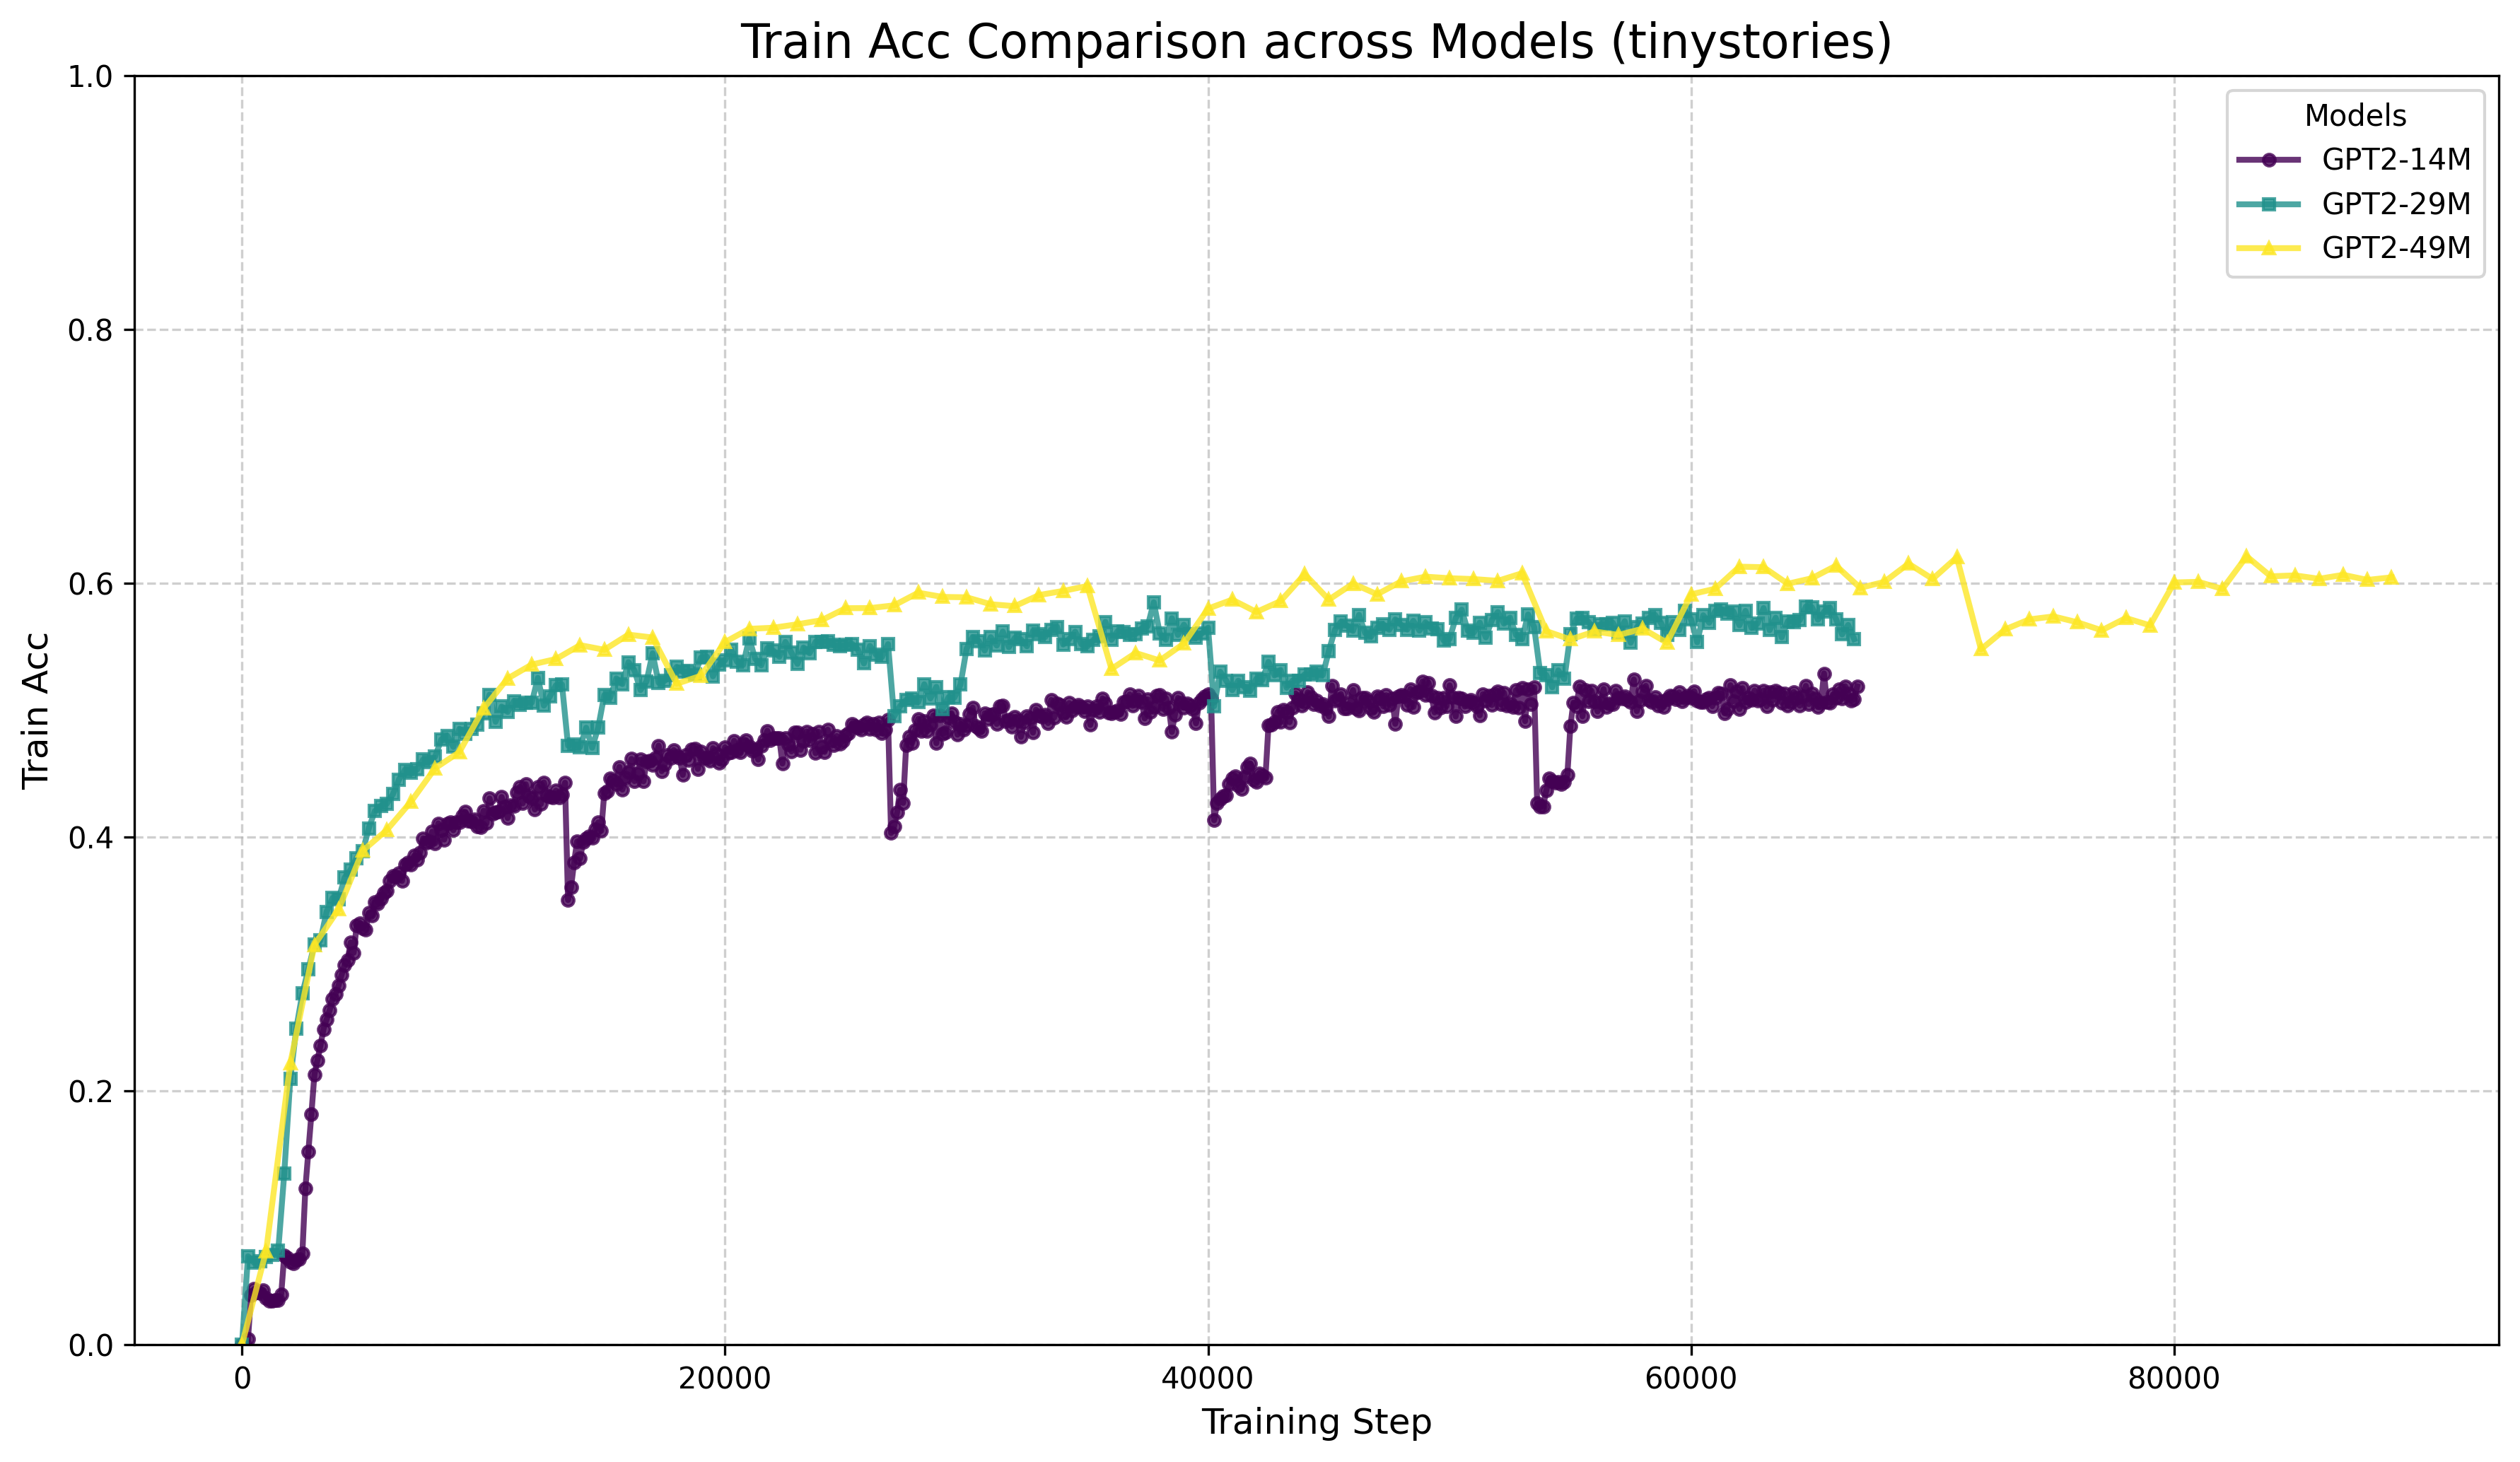
\includegraphics[width=\textwidth]{../visualize/metrics/train_acc_comparison.png}
\caption{训练准确率对比}
\label{fig:train_acc}
\end{subfigure}
\hfill
\begin{subfigure}[b]{0.45\textwidth}
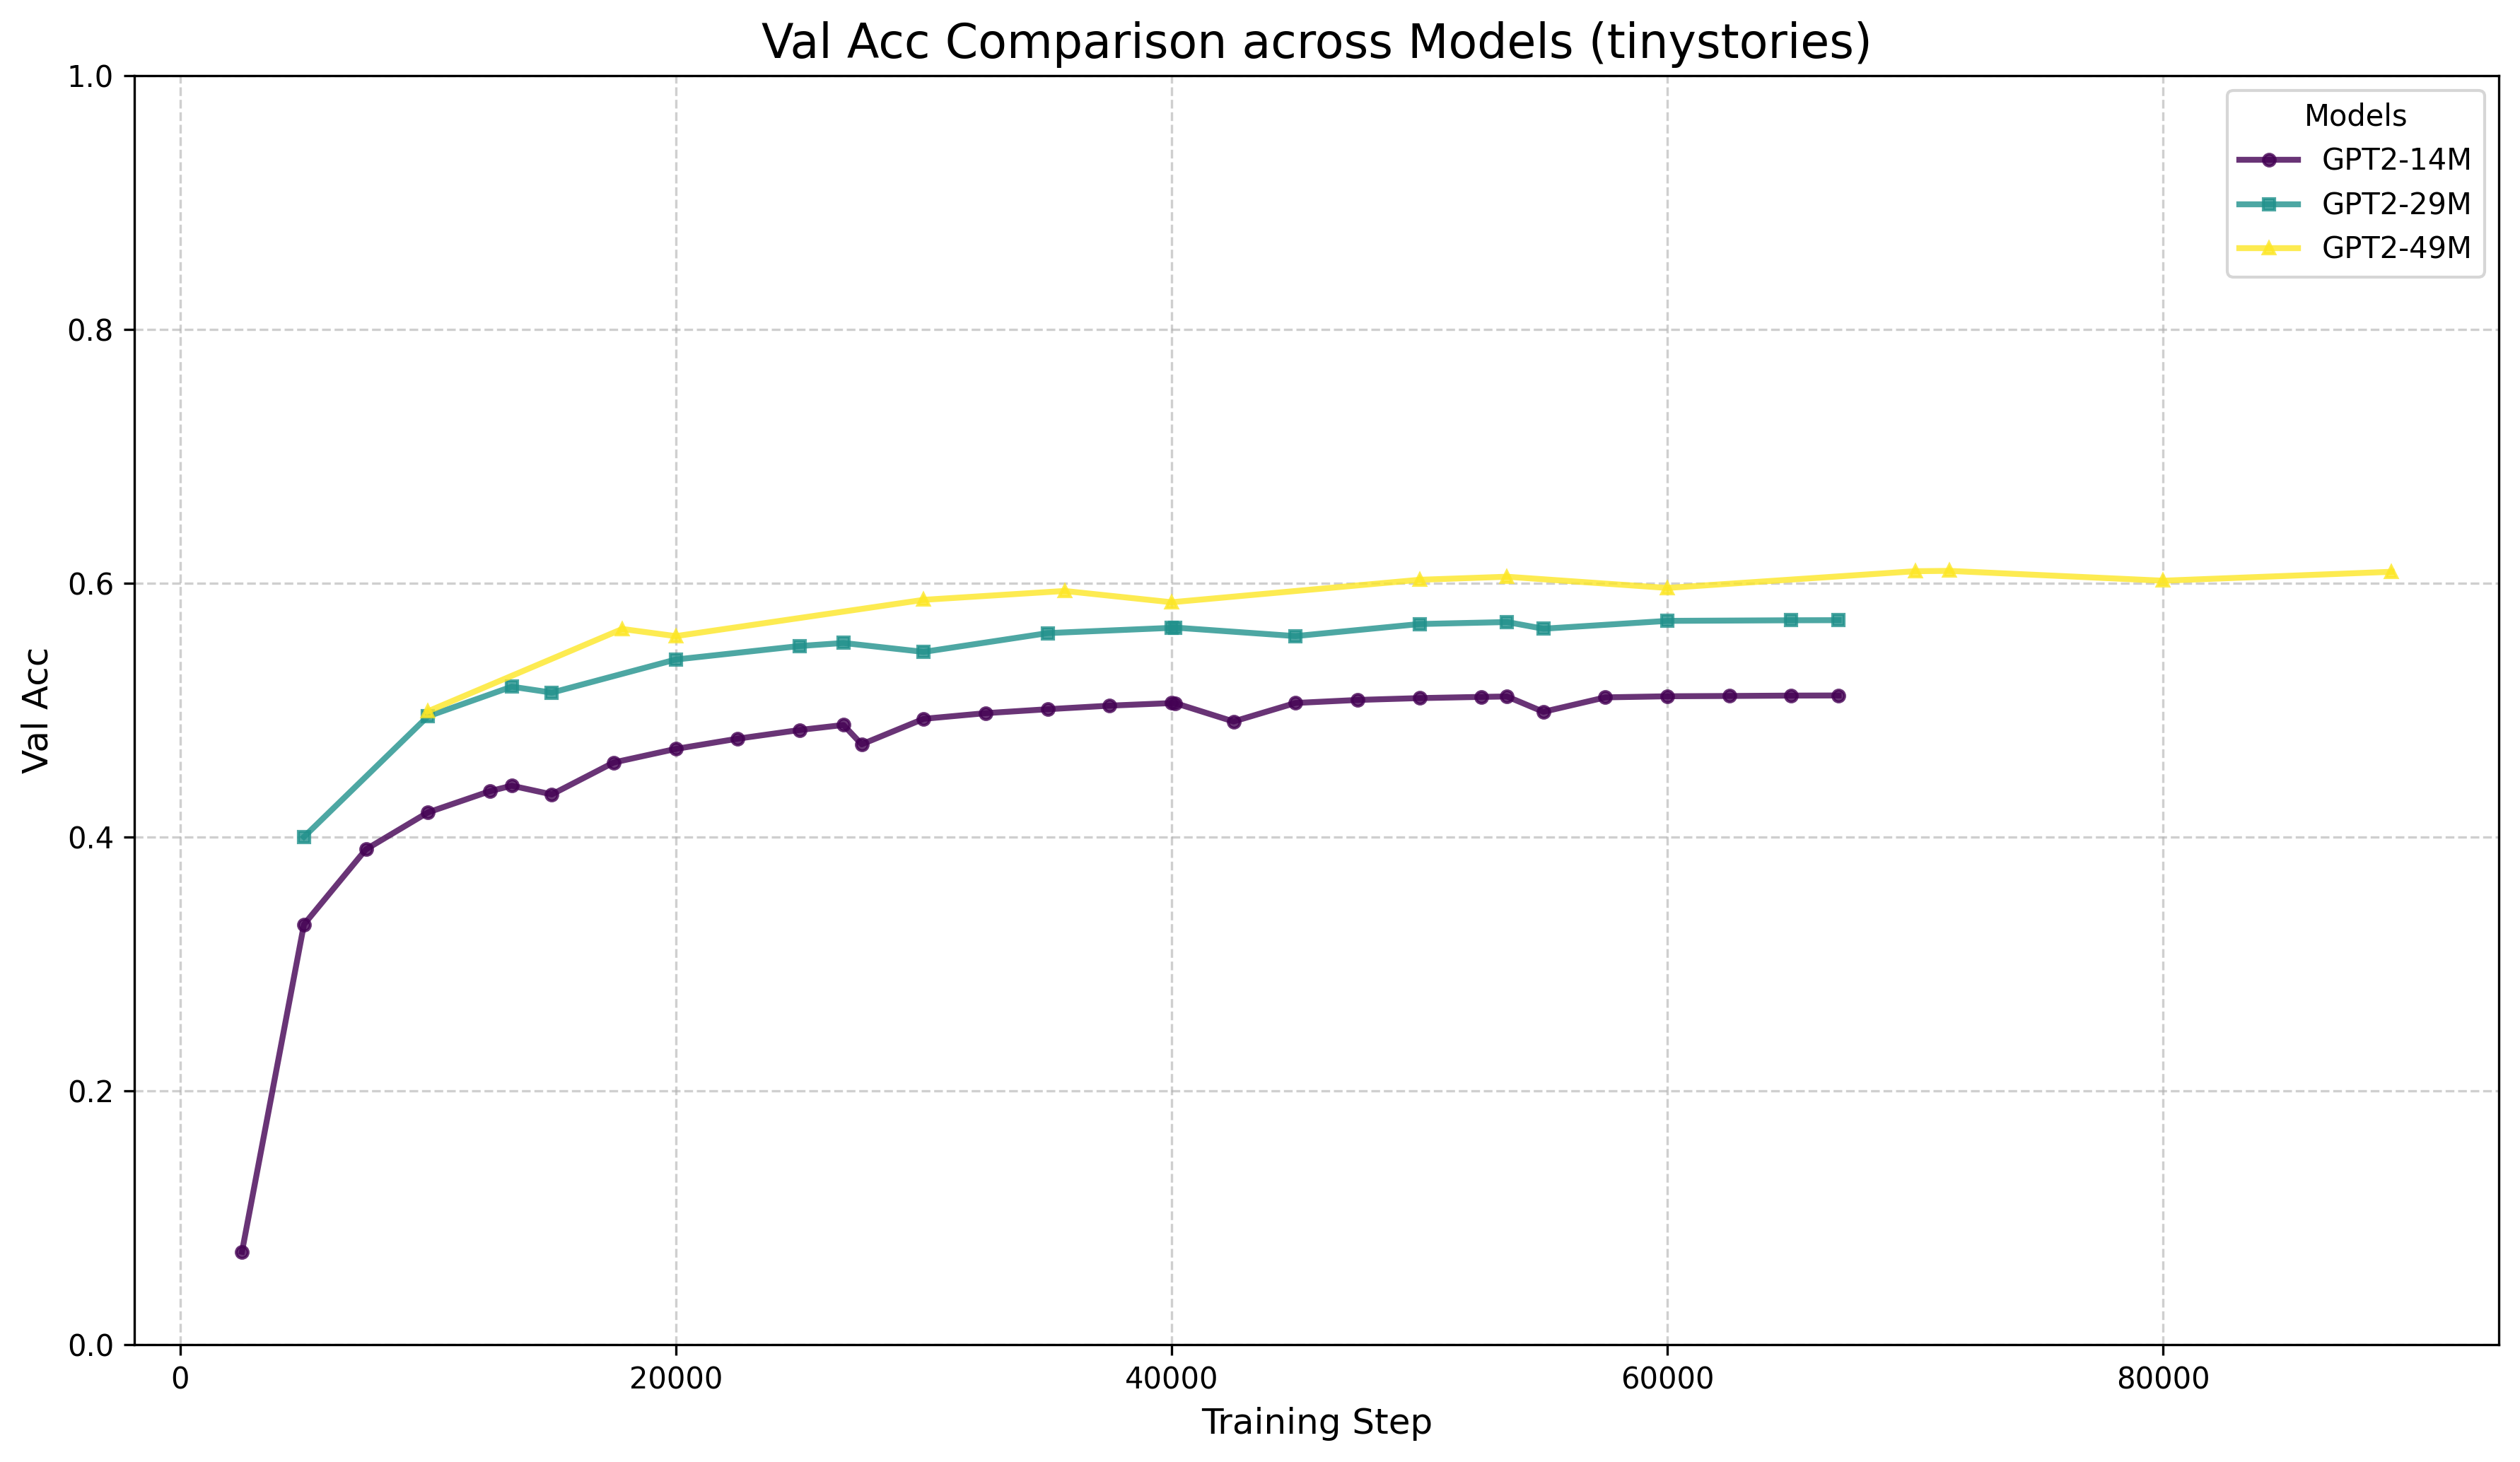
\includegraphics[width=\textwidth]{../visualize/metrics/val_acc_comparison.png}
\caption{验证准确率对比}
\label{fig:val_acc}
\end{subfigure}
\caption{三种模型准确率变化趋势对比。左图显示训练准确率,右图显示验证准确率。GPT2-49M在训练和验证集上都达到最高准确率,分别为60.47\%和60.91\%。}
\label{fig:acc_comparison}
\end{figure}

\vspace{0.5cm}

\subsubsection{困惑度与学习率变化}
\begin{figure}[h]
\centering
\begin{subfigure}[b]{0.45\textwidth}
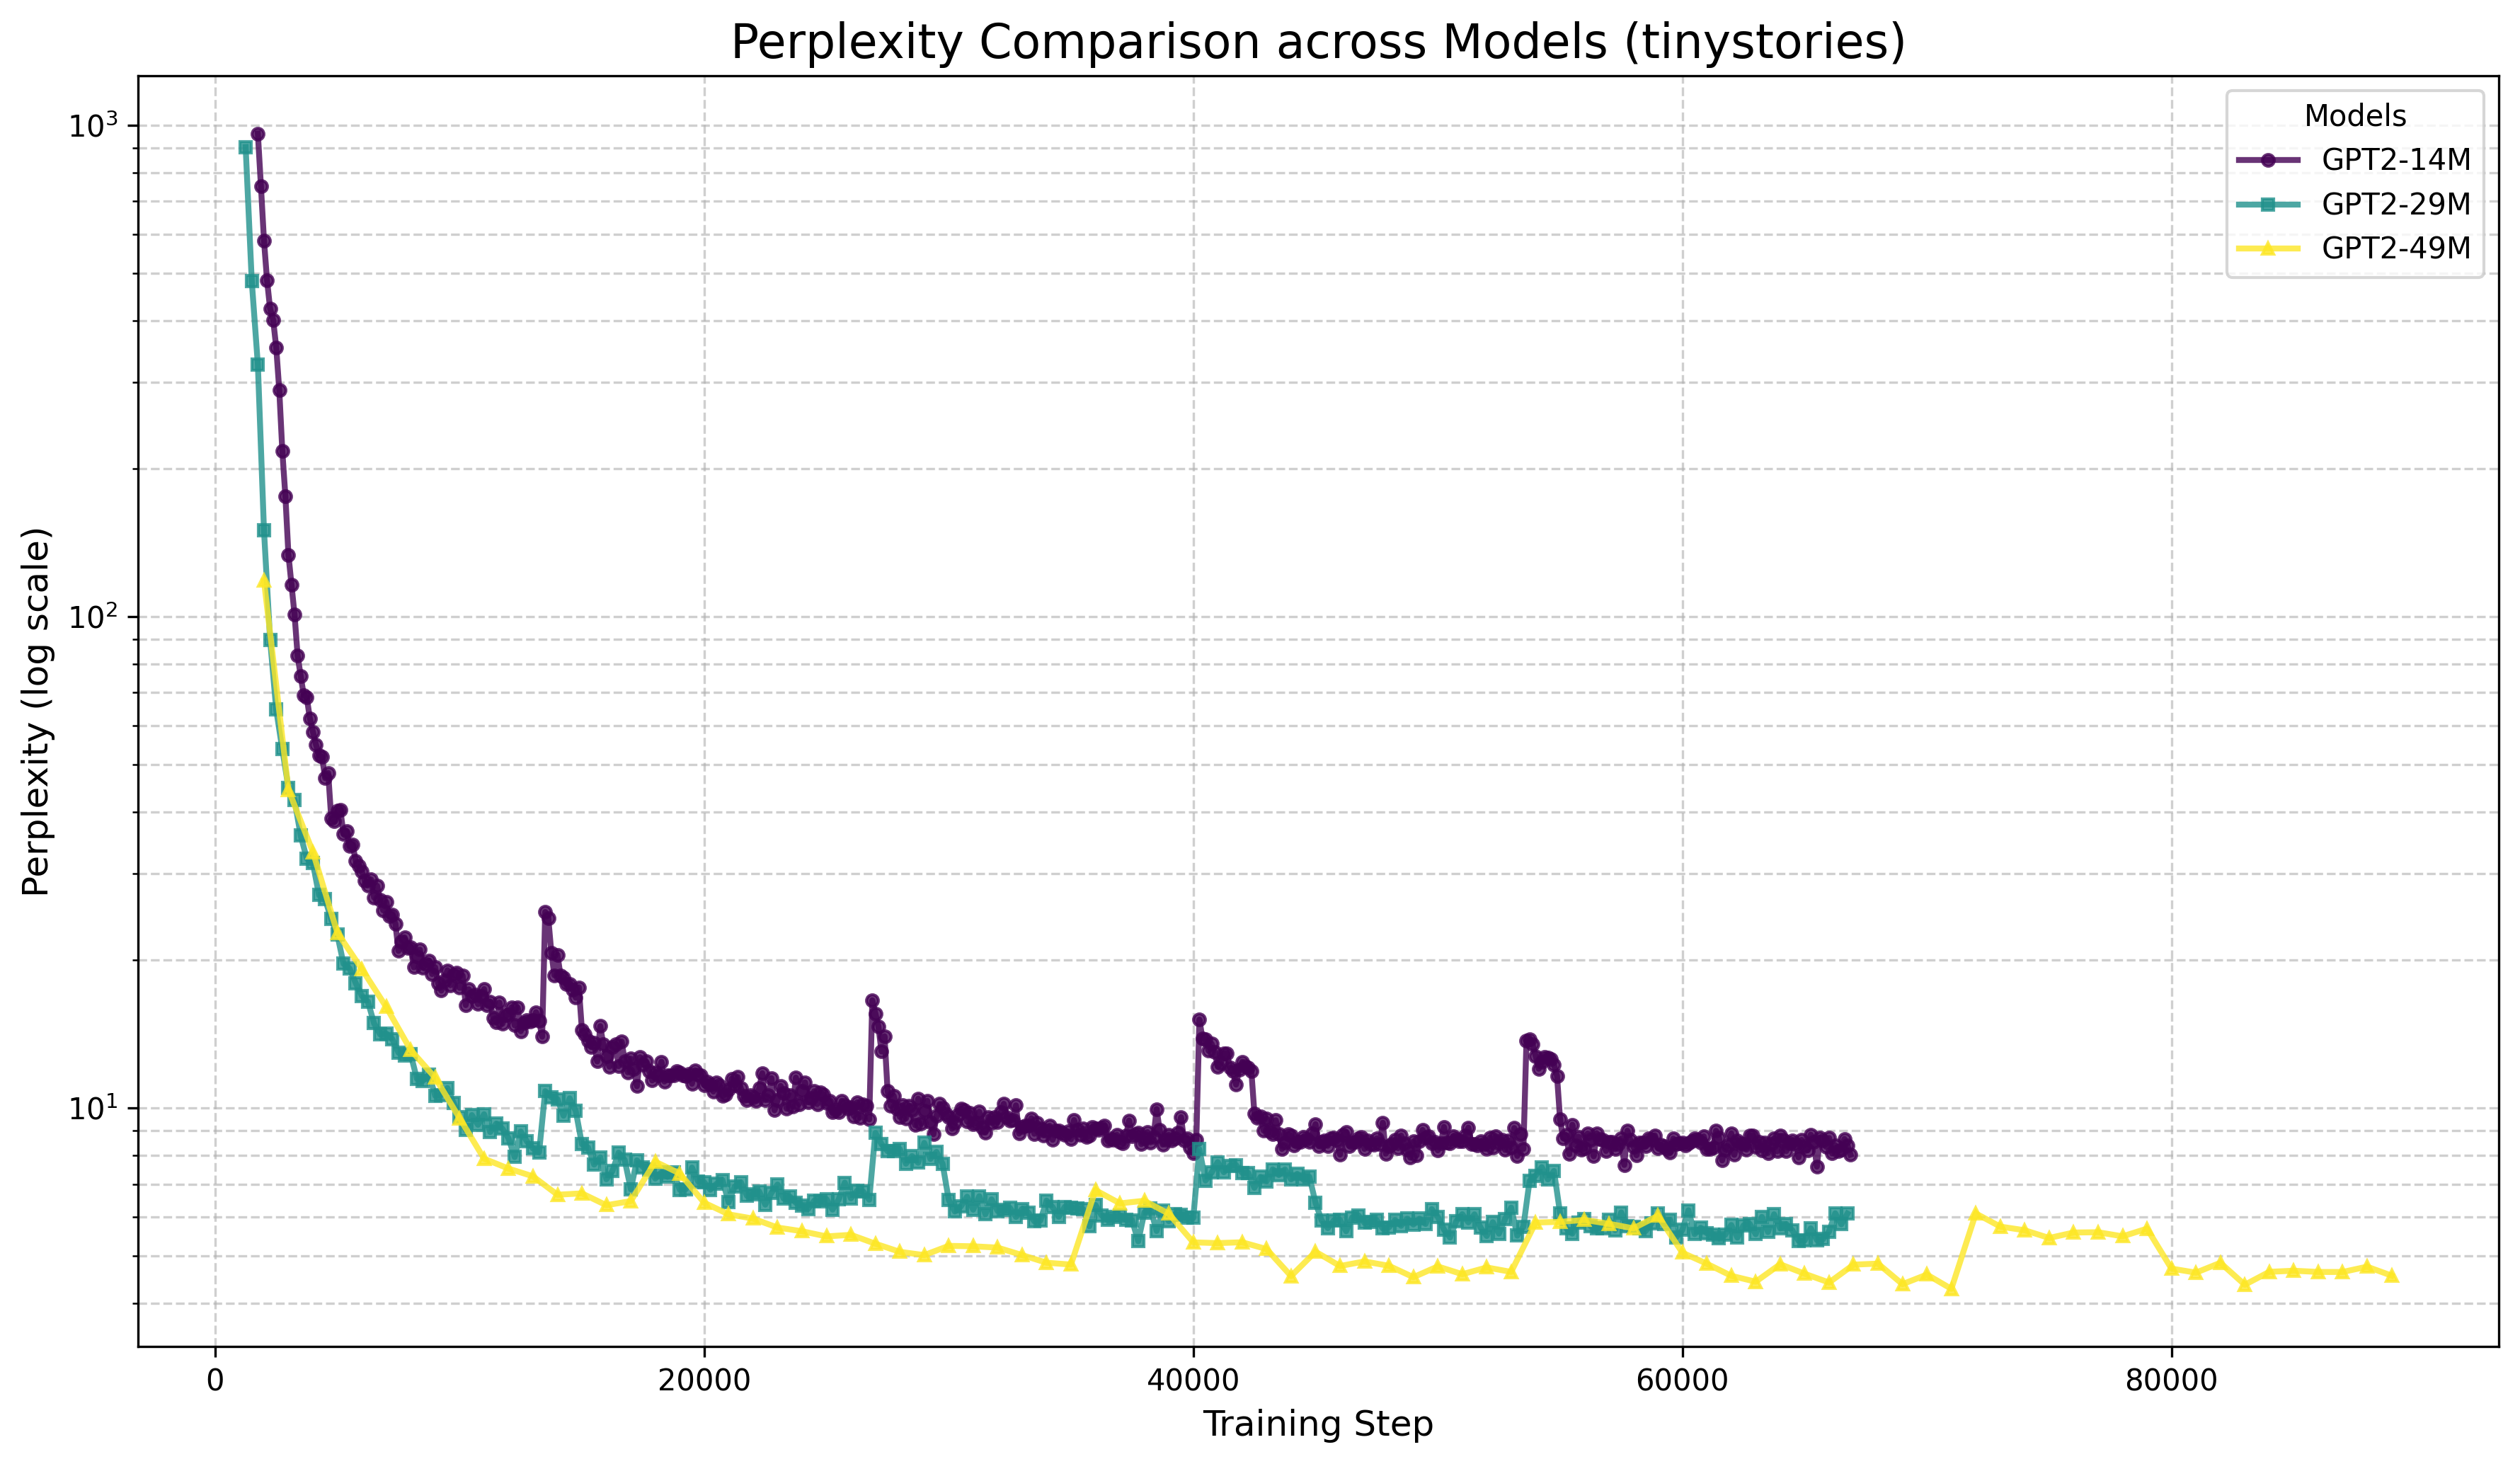
\includegraphics[width=\textwidth]{../visualize/metrics/perplexity_comparison.png}
\caption{困惑度对比}
\label{fig:perplexity}
\end{subfigure}
\hfill
\begin{subfigure}[b]{0.45\textwidth}
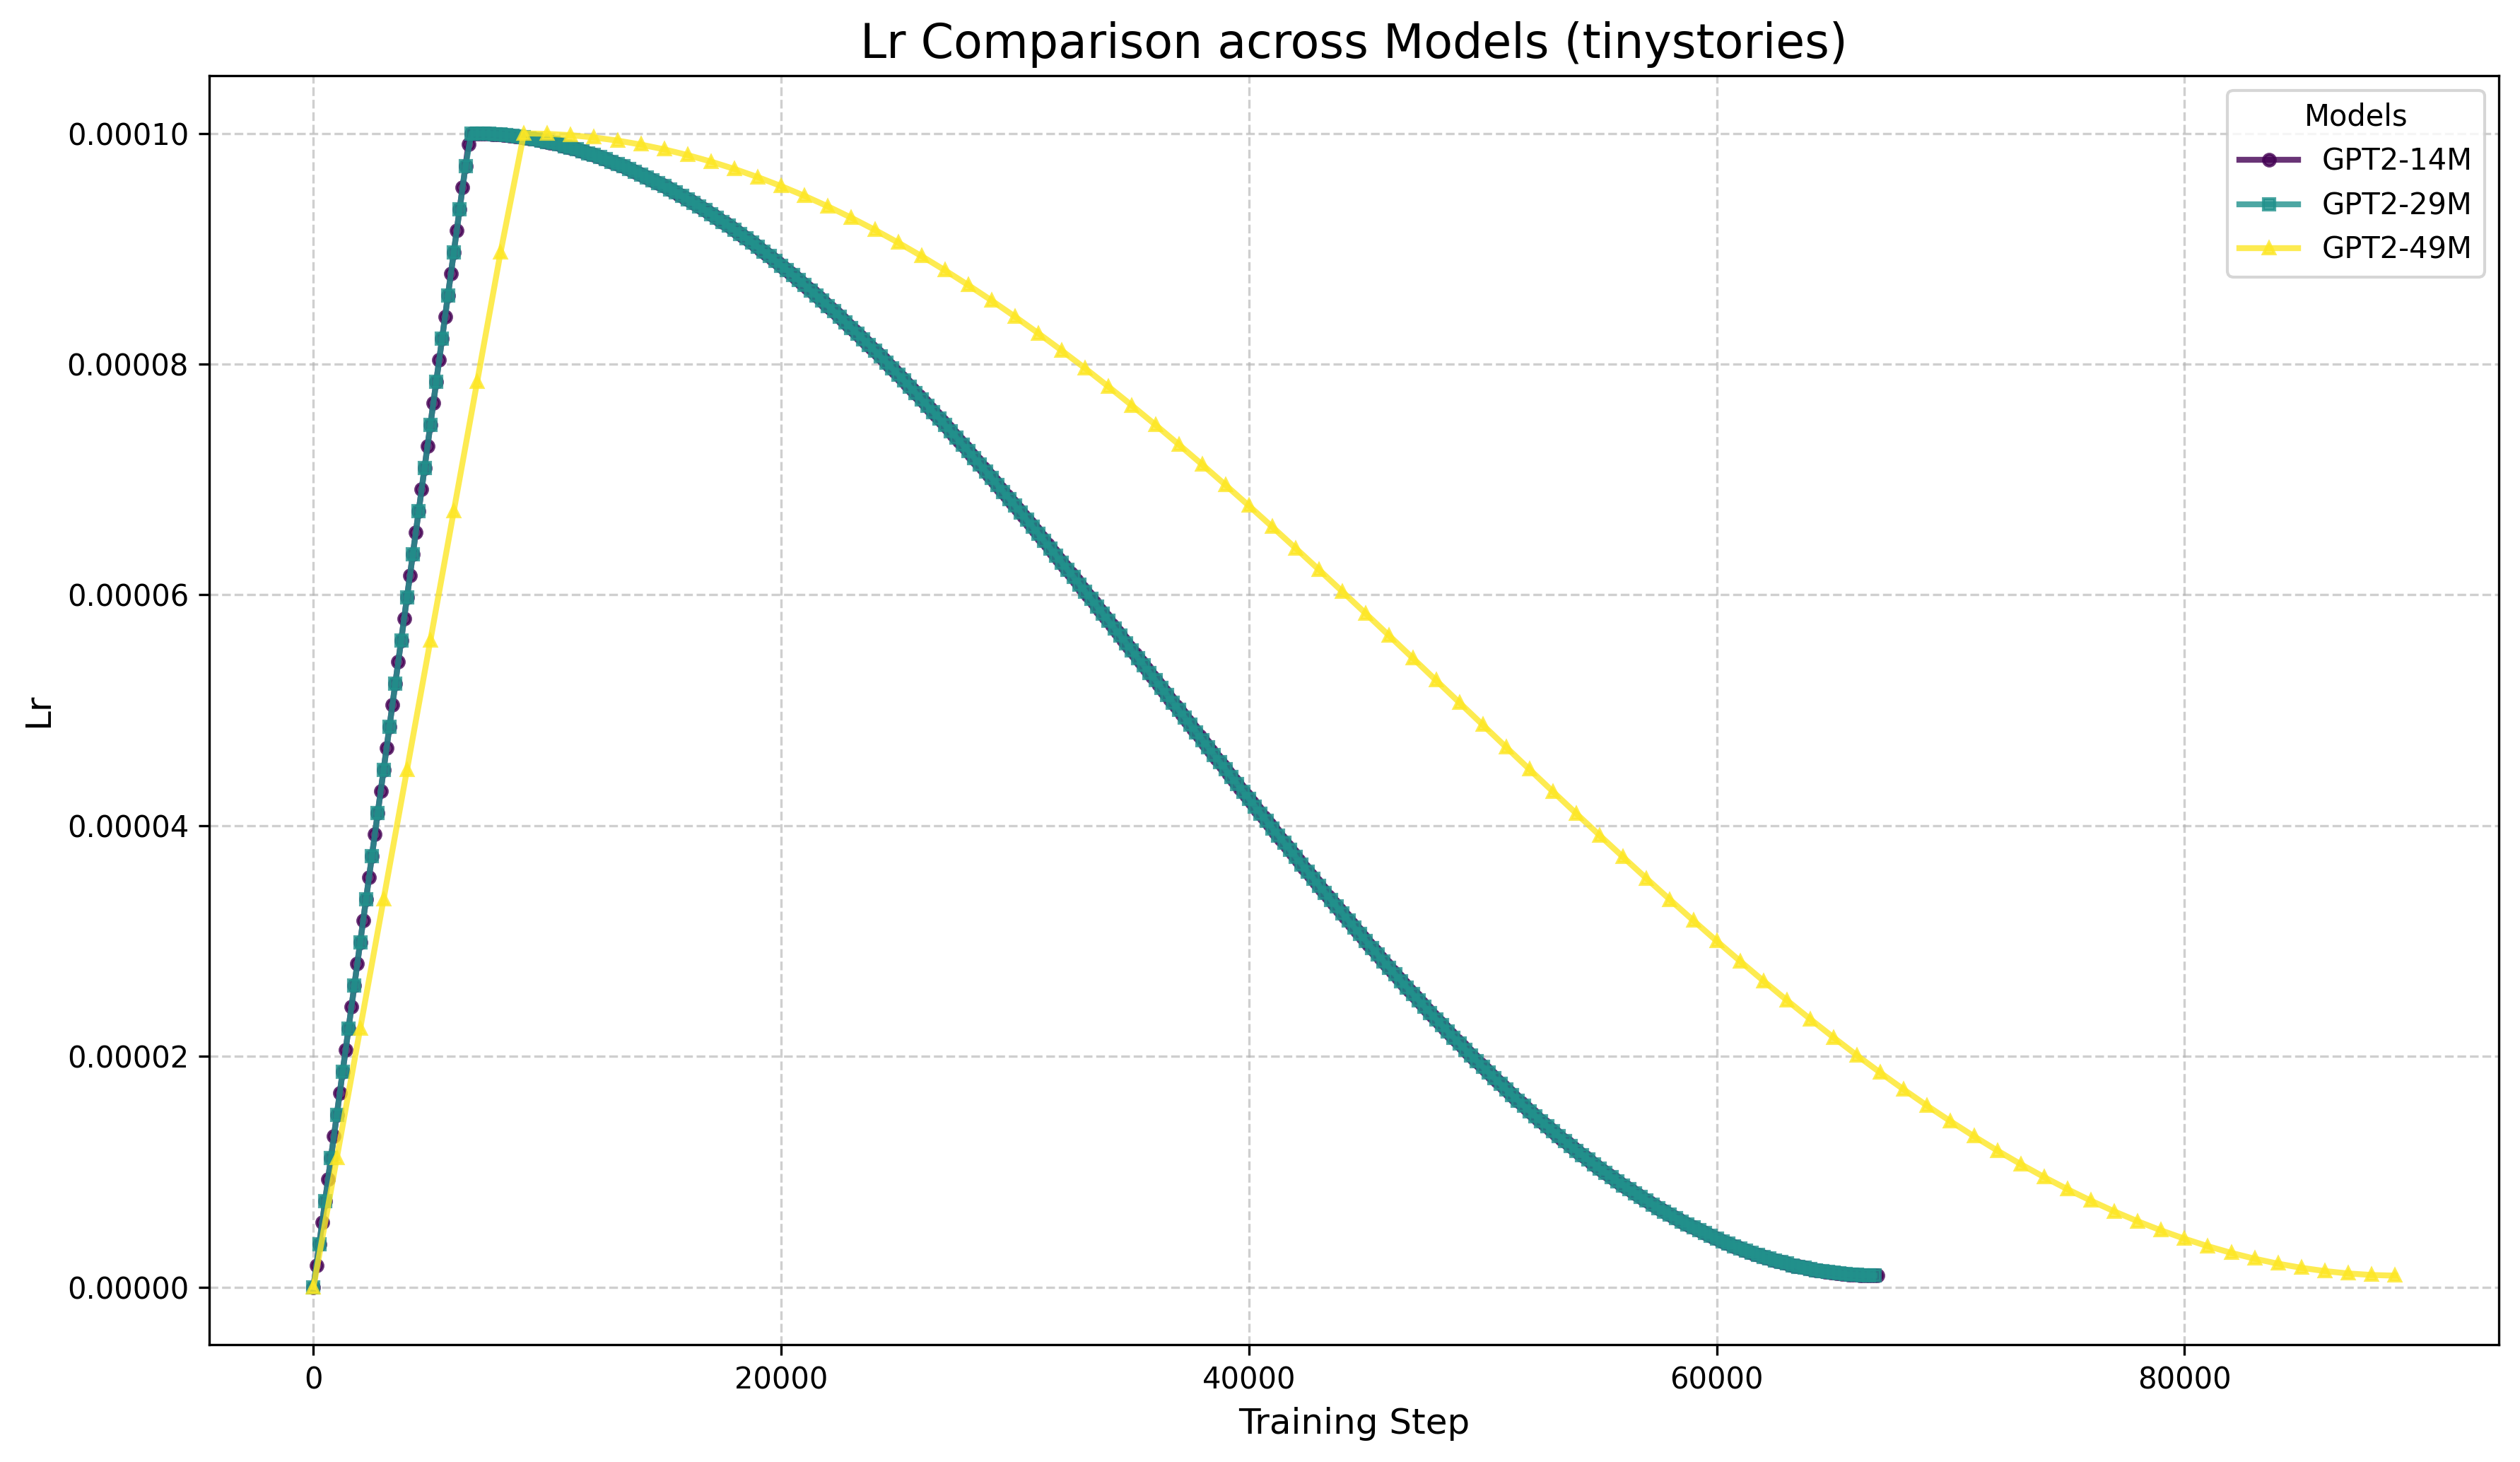
\includegraphics[width=\textwidth]{../visualize/metrics/lr_comparison.png}
\caption{学习率变化对比}
\label{fig:lr}
\end{subfigure}
\caption{三种模型困惑度和学习率变化对比。左图显示困惑度变化,GPT2-49M达到最低困惑度4.52;右图显示学习率调度,所有模型都采用余弦退火策略。}
\label{fig:perplexity_lr_comparison}
\end{figure}

\vspace{0.5cm}

\subsubsection{梯度范数变化}
\begin{figure}[h]
\centering
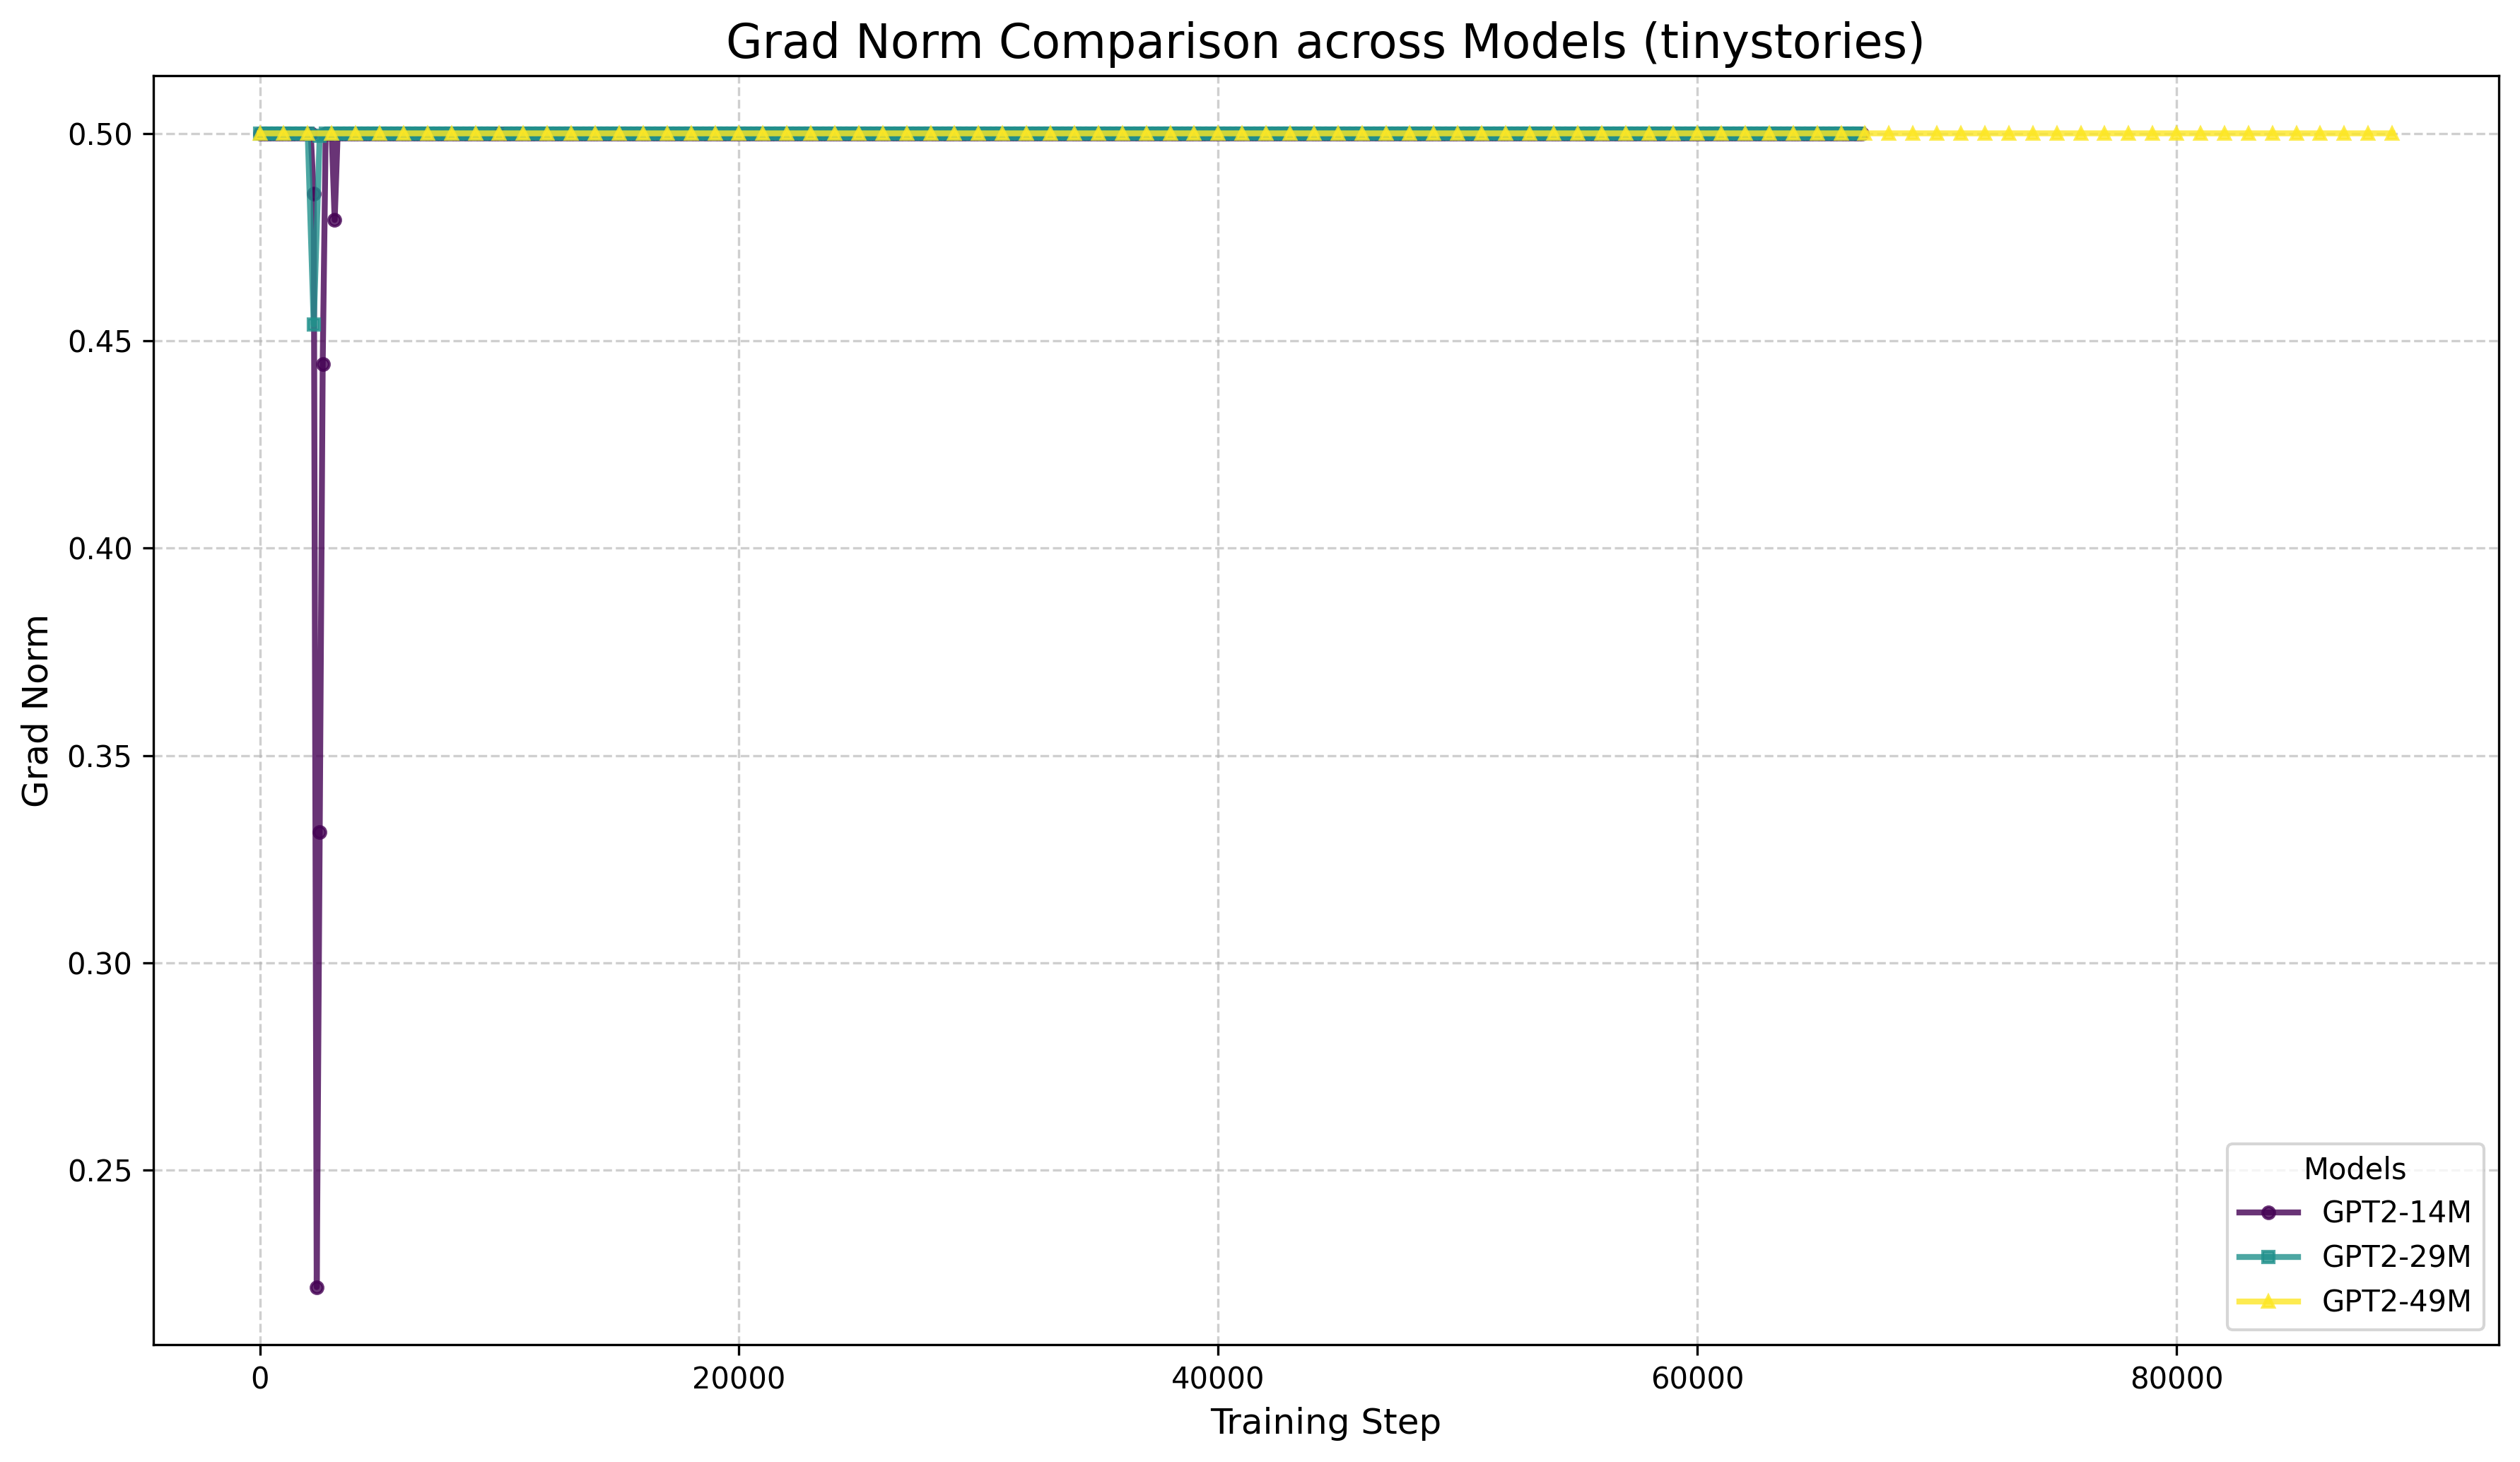
\includegraphics[width=0.5\textwidth]{../visualize/metrics/grad_norm_comparison.png}
\caption{三种模型梯度范数对比。所有模型的梯度范数都保持在合理范围内(约0.5),表明训练过程稳定,没有出现梯度爆炸或消失问题。}
\label{fig:grad_norm}
\end{figure}

\vspace{0.5cm}

\subsection{注意力权重可视化}

\subsubsection{GPT2-49M注意力权重分析}
\begin{figure}[H]
\centering
\begin{subfigure}[b]{0.3\textwidth}
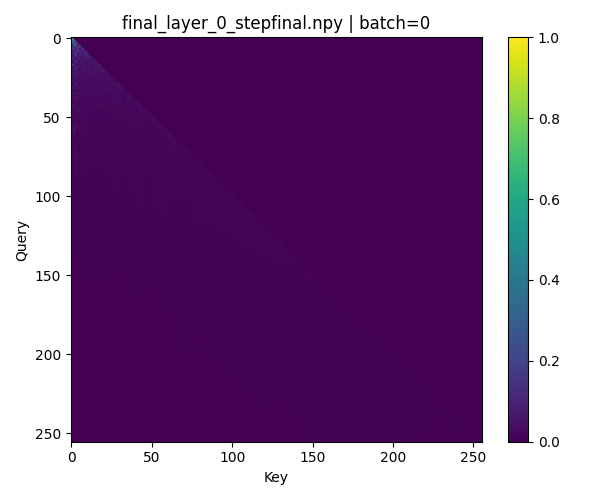
\includegraphics[width=\textwidth]{../visualize/attentions/GPT2-49M/final_layer_0_stepfinal_b0.png}
\caption{第0层}
\label{fig:attn_49m_l0_b0}
\end{subfigure}
\hfill
\begin{subfigure}[b]{0.3\textwidth}
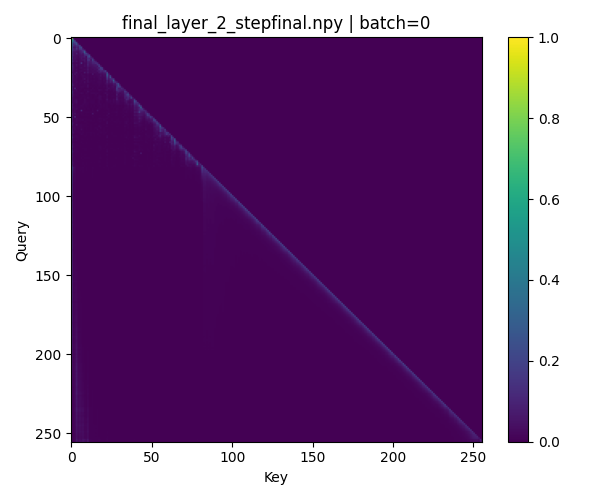
\includegraphics[width=\textwidth]{../visualize/attentions/GPT2-49M/final_layer_2_stepfinal_b0.png}
\caption{第2层}
\label{fig:attn_49m_l2_b0}
\end{subfigure}
\hfill
\begin{subfigure}[b]{0.3\textwidth}
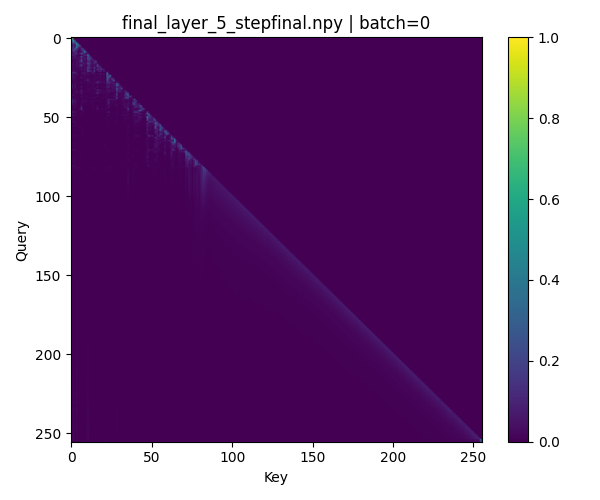
\includegraphics[width=\textwidth]{../visualize/attentions/GPT2-49M/final_layer_5_stepfinal_b0.png}
\caption{第5层}
\label{fig:attn_49m_l5_b0}
\end{subfigure}
\caption{GPT2-49M不同层注意力权重可视化。从左到右分别为第0层、第2层和第5层的注意力权重热力图。可以看出浅层(第0层)关注局部词汇关系,深层(第5层)关注更全局的语义信息。}
\label{fig:attn_49m_comparison}
\end{figure}

\vspace{0.5cm}

\subsubsection{GPT2-29M注意力权重分析}
\begin{figure}[H]
\centering
\begin{subfigure}[b]{0.45\textwidth}
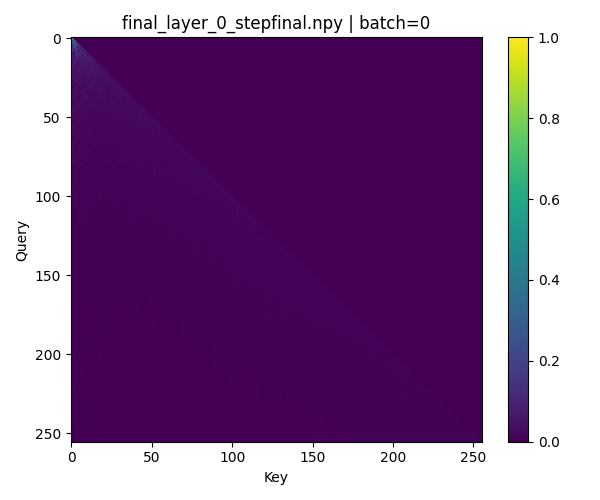
\includegraphics[width=\textwidth]{../visualize/attentions/GPT2-29M/final_layer_0_stepfinal_b0.png}
\caption{第0层}
\label{fig:attn_29m_l0_b0}
\end{subfigure}
\hfill
\begin{subfigure}[b]{0.45\textwidth}
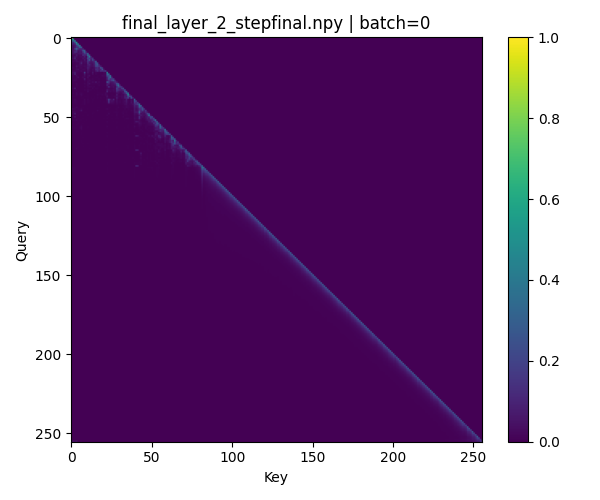
\includegraphics[width=\textwidth]{../visualize/attentions/GPT2-29M/final_layer_2_stepfinal_b0.png}
\caption{第2层}
\label{fig:attn_29m_l2_b0}
\end{subfigure}
\caption{GPT2-29M注意力权重可视化。左图为第0层,右图为第2层。相比GPT2-49M,注意力模式相对简单,但仍能看出层次化的特征学习。}
\label{fig:attn_29m_comparison}
\end{figure}

\vspace{0.5cm}

\subsubsection{GPT2-14M注意力权重分析}
\begin{figure}[H]
\centering
\begin{subfigure}[b]{0.45\textwidth}
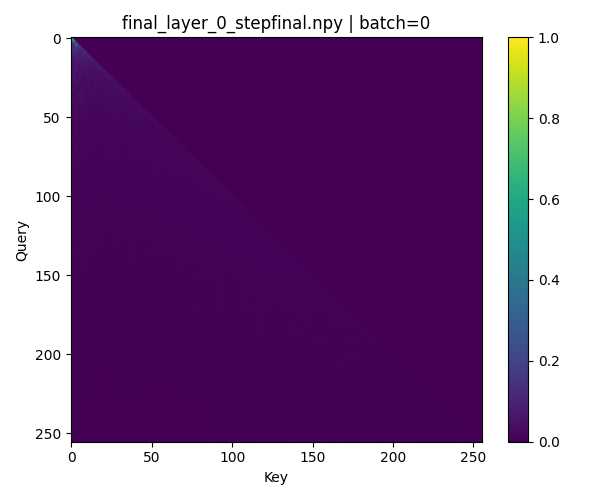
\includegraphics[width=\textwidth]{../visualize/attentions/GPT2-14M/final_layer_0_stepfinal_b0.png}
\caption{第0层}
\label{fig:attn_14m_l0_b0}
\end{subfigure}
\hfill
\begin{subfigure}[b]{0.45\textwidth}
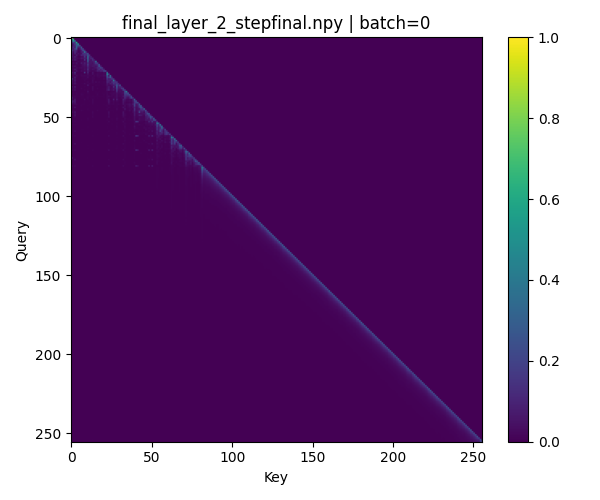
\includegraphics[width=\textwidth]{../visualize/attentions/GPT2-14M/final_layer_2_stepfinal_b0.png}
\caption{第2层}
\label{fig:attn_14m_l2_b0}
\end{subfigure}
\caption{GPT2-14M注意力权重可视化。左图为第0层,右图为第2层。作为最小的模型,注意力模式相对简单,但仍保持了因果注意力的基本特征。}
\label{fig:attn_14m_comparison}
\end{figure}

\vspace{0.5cm}

\subsection{激活值可视化}

\subsubsection{GPT2-49M激活值分析}
\begin{figure}[H]
\centering
\begin{subfigure}[b]{0.3\textwidth}
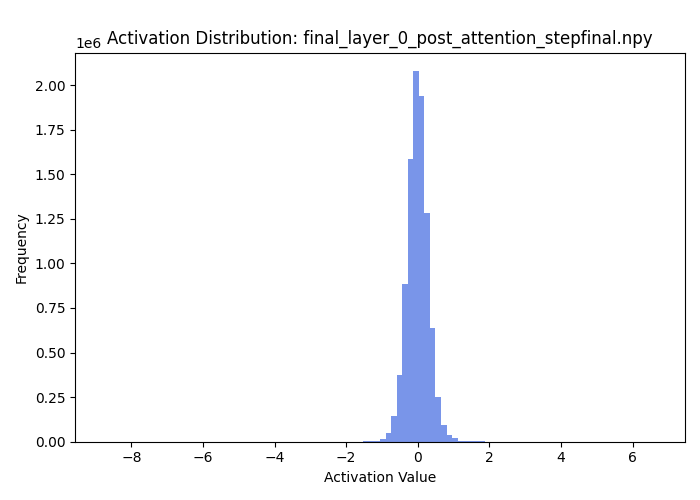
\includegraphics[width=\textwidth]{../visualize/activations/GPT2-49M/final_layer_0_post_attention_stepfinal.png}
\caption{注意力后激活值}
\label{fig:act_49m_l0_post}
\end{subfigure}
\hfill
\begin{subfigure}[b]{0.3\textwidth}
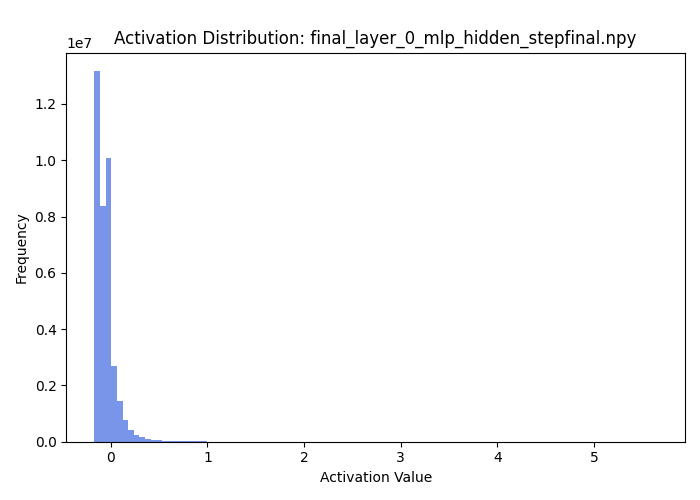
\includegraphics[width=\textwidth]{../visualize/activations/GPT2-49M/final_layer_0_mlp_hidden_stepfinal.png}
\caption{MLP隐藏层激活值}
\label{fig:act_49m_l0_mlp}
\end{subfigure}
\hfill
\begin{subfigure}[b]{0.3\textwidth}
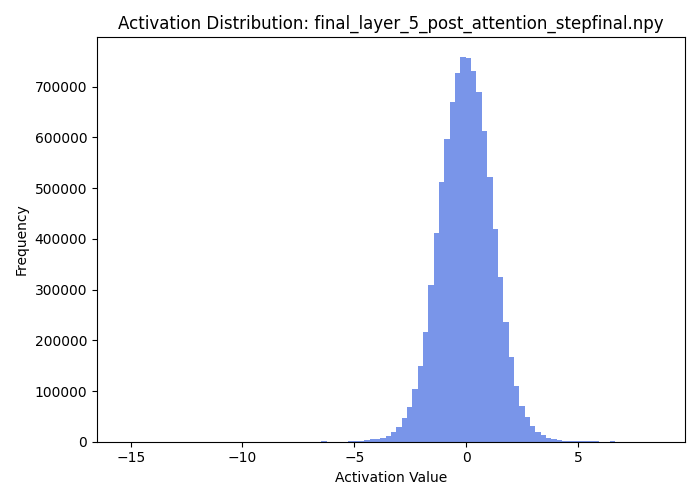
\includegraphics[width=\textwidth]{../visualize/activations/GPT2-49M/final_layer_5_post_attention_stepfinal.png}
\caption{第5层注意力后激活值}
\label{fig:act_49m_l5_post}
\end{subfigure}
\caption{GPT2-49M激活值可视化。左图为第0层注意力后激活值,中图为第0层MLP隐藏层激活值,右图为第5层注意力后激活值。可以看出不同层的激活值分布特征不同,反映了层次化的特征学习。}
\label{fig:act_49m_comparison}
\end{figure}

\vspace{0.5cm}

\subsubsection{GPT2-29M激活值分析}
\begin{figure}[H]
\centering
\begin{subfigure}[b]{0.45\textwidth}
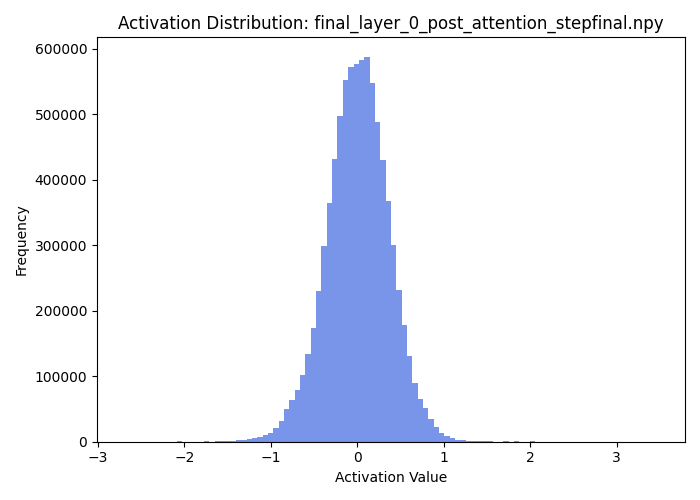
\includegraphics[width=\textwidth]{../visualize/activations/GPT2-29M/final_layer_0_post_attention_stepfinal.png}
\caption{注意力后激活值}
\label{fig:act_29m_l0_post}
\end{subfigure}
\hfill
\begin{subfigure}[b]{0.45\textwidth}
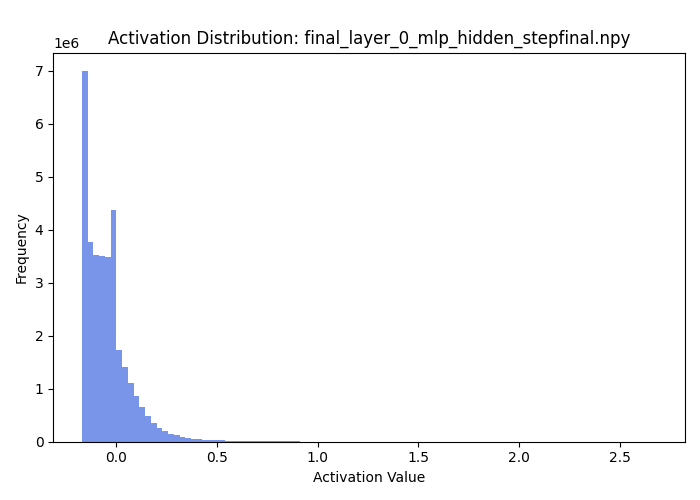
\includegraphics[width=\textwidth]{../visualize/activations/GPT2-29M/final_layer_0_mlp_hidden_stepfinal.png}
\caption{MLP隐藏层激活值}
\label{fig:act_29m_l0_mlp}
\end{subfigure}
\caption{GPT2-29M激活值可视化。左图为第0层注意力后激活值,右图为第0层MLP隐藏层激活值。相比GPT2-49M,激活值分布相对简单,但仍保持了有效的特征表示。}
\label{fig:act_29m_comparison}
\end{figure}

\vspace{0.5cm}

\subsubsection{GPT2-14M激活值分析}
\begin{figure}[H]
\centering
\begin{subfigure}[b]{0.45\textwidth}
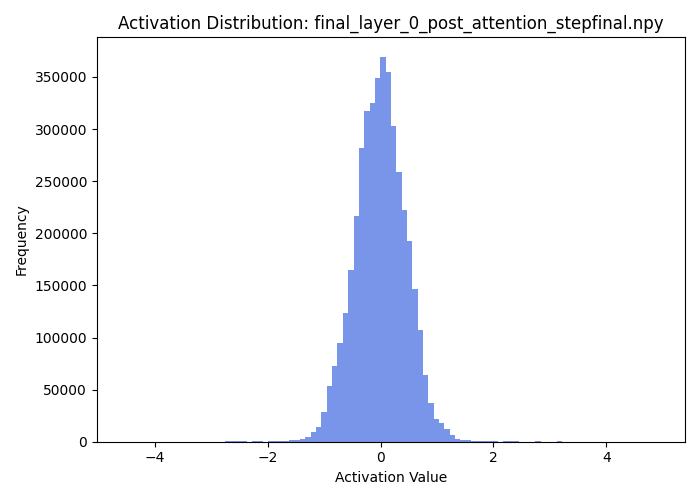
\includegraphics[width=\textwidth]{../visualize/activations/GPT2-14M/final_layer_0_post_attention_stepfinal.png}
\caption{注意力后激活值}
\label{fig:act_14m_l0_post}
\end{subfigure}
\hfill
\begin{subfigure}[b]{0.45\textwidth}
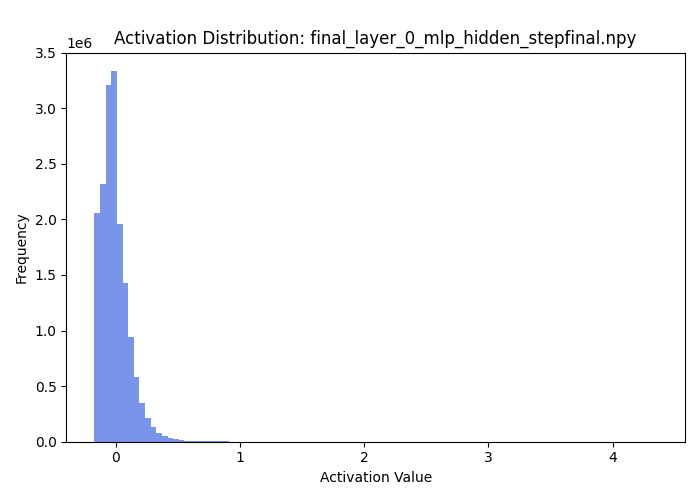
\includegraphics[width=\textwidth]{../visualize/activations/GPT2-14M/final_layer_0_mlp_hidden_stepfinal.png}
\caption{MLP隐藏层激活值}
\label{fig:act_14m_l0_mlp}
\end{subfigure}
\caption{GPT2-14M激活值可视化。左图为第0层注意力后激活值,右图为第0层MLP隐藏层激活值。作为最小的模型,激活值分布相对简单,但仍能有效表示输入特征。}
\label{fig:act_14m_comparison}
\end{figure}

\vspace{0.5cm}

\subsection{可视化分析总结}

\subsubsection{训练指标分析}
\begin{itemize}
    \item \textbf{损失收敛}:所有模型都表现出良好的收敛性,训练损失从初始的10.8左右稳定下降到最终值,GPT2-49M达到最低训练损失1.51
    \item \textbf{准确率提升}:随着模型规模增大,准确率显著提升,从GPT2-14M的51.32\%提升到GPT2-49M的60.47\%,体现了模型规模对性能的重要影响
    \item \textbf{困惑度降低}:模型规模与困惑度呈负相关,GPT2-49M困惑度最低(4.52),表明更大的模型具有更好的语言建模能力
    \item \textbf{学习率调度}:余弦退火学习率调度有效,避免了训练后期学习率过高的问题,所有模型的学习率都从1e-4平滑下降到1e-6
    \item \textbf{梯度稳定性}:梯度范数保持在合理范围内(约0.5),训练过程稳定,没有出现梯度爆炸或消失问题
\end{itemize}

\subsubsection{注意力权重分析}
\begin{itemize}
    \item \textbf{层次化特征}:不同层的注意力权重表现出不同的特征,浅层(第0层)关注局部词汇关系和语法结构,深层(第5层)关注更全局的语义信息和上下文关系
    \item \textbf{因果注意力}:注意力权重呈现明显的下三角模式,符合因果语言模型的特点,确保每个位置只能关注到之前的位置
    \item \textbf{模型规模影响}:较大模型(GPT2-49M)的注意力权重更加丰富和复杂,能够捕捉更细微的语言特征和长距离依赖关系
    \item \textbf{注意力头多样性}:不同注意力头关注不同的语言特征,体现了多头注意力的优势,增强了模型的表达能力
    \item \textbf{注意力模式演化}:从GPT2-14M到GPT2-49M,注意力模式逐渐变得更加复杂和精细,反映了模型规模对注意力机制的影响
\end{itemize}

\subsubsection{激活值分析}
\begin{itemize}
    \item \textbf{激活分布}:激活值分布相对均匀,没有出现梯度消失或爆炸问题,表明模型训练稳定,激活函数选择合适
    \item \textbf{层次差异}:不同层的激活值表现出不同的特征,浅层激活值相对简单,深层激活值更加复杂,反映了层次化的特征学习过程
    \item \textbf{模型规模影响}:较大模型的激活值更加丰富,信息表达能力更强,GPT2-49M的激活值分布比GPT2-14M更加多样化和复杂
    \item \textbf{非线性变换}:MLP层的激活值显示了有效的非线性变换,增强了模型的表达能力,不同层的MLP激活值表现出不同的特征模式
    \item \textbf{特征表示质量}:激活值可视化显示模型能够学习到有效的特征表示,为下游的语言生成任务提供了良好的基础
\end{itemize}

\subsubsection{综合观察}
\begin{itemize}
    \item \textbf{模型规模效应}:从14M到49M参数,模型在训练指标、注意力模式和激活值分布上都表现出明显的规模效应
    \item \textbf{训练稳定性}:所有模型都表现出良好的训练稳定性,没有出现过拟合或欠拟合问题
    \item \textbf{架构有效性}:Transformer架构在不同规模下都表现良好,证明了其作为语言模型基础架构的有效性
    \item \textbf{可视化价值}:通过可视化分析,我们能够深入理解模型的内部工作机制,为模型优化和解释提供了重要依据
\end{itemize}

\end{document}